% The English tutorial as a document of its own, with English prefixes (Figure,
% Table, Chapter, Section). Build it with `make compile-en`, which first writes
% .tw-thesis-build/config-en.tex from contents/i18n/en/config.yml. Your thesis is
% built from main.tex; this file is not part of it.
\def\twgenerated{.tw-thesis-build/config-en.tex}
\documentclass{tw-thesis}

\begin{document}

\thesisfront

\chapter{Getting Started}\label{cha:start}

On first use, keep the sample files as they are and go through the steps in this chapter once: compile, confirm that a PDF is produced, and check that the fonts and pages display correctly. Then fill in your own thesis details and replace the titles and text chapter by chapter. Recompile after every change, so that if an error appears it is easy to tell which edit caused it.

The source files of this tutorial all live in \code{contents/}, and each chapter there corresponds to a chapter in the PDF. When you see a figure, citation or code layout you want, open the matching chapter, copy the example, and swap in your own text and data. Leave syntax you are unsure about as it is, adjust it step by step against the compiled result, and reuse it in other chapters once it works.

\section{Installing and Compiling}

Before compiling and writing, install a \LaTeX{} distribution. The template is compiled with \XeLaTeX{}; pick \href{https://www.tug.org/texlive/}{TeX Live} (MacTeX on macOS, the TeX Live installer on Windows) or the lighter \href{https://yihui.org/tinytex/}{TinyTeX}. The lines below are different ways to install one; run whichever fits your system. \code{brew} and \code{winget} must already be installed.

\begin{lstlisting}[language=bash]
brew install --cask mactex-no-gui   # macOS
winget install --id MiKTeX.MiKTeX   # Windows
sudo apt install texlive-full       # Debian / Ubuntu
\end{lstlisting}

The small program that converts the config file, \code{scripts/gen.lua}, is run by the \code{texlua} that comes with \TeX{}, so you do not need to install Python or anything else. References use the \code{citation-style-language} package; a full \TeX{} Live already includes it, and with TinyTeX or a partial install you add it yourself:

\begin{lstlisting}[language=bash]
tlmgr install citation-style-language
\end{lstlisting}

Once installed, switch to the project root in a terminal, which is the folder that contains \code{main.tex}, and run:

\begin{lstlisting}[language=bash]
texlua scripts/gen.lua
latexmk -xelatex main.tex
\end{lstlisting}

The first line reads \code{config.yml} and the school settings and writes \code{.tw-thesis-config.tex}. \LaTeX{} cannot read YAML directly, so this has to be repeated after every change to the config file. The second line is the actual compile; when it finishes, \code{main.pdf} appears in the same folder. Open the PDF and check that Chinese displays correctly. The fonts shipped with the project sit in \code{fonts/} and are loaded by file from \code{tw-thesis.cls}, so there is no need to install them on the system.

If \code{make} is installed, the two lines above shrink to the following commands, which run the jobs defined in the project's \code{Makefile}:

\begin{lstlisting}[language=bash]
make            # write main.pdf (draft, no watermark)
make watch      # recompile on every save
make release    # final version, with the school watermark
make clean      # delete main.pdf and the build leftovers
\end{lstlisting}

While writing, run \code{make watch} in the project root to start \textbf{watch mode}. The command keeps watching the files; every time you edit and save the thesis text or the settings, \code{latexmk} recompiles and updates the same \code{main.pdf}, so you never have to run the compile command by hand. Keep that terminal open while you work, and press \code{Ctrl+C} to stop watching.

To produce a version with a watermark, stop watch mode first and then run \code{make release}. It adds

\begin{lstlisting}[language=bash]
-usepretex='\def\twwatermark{1}'
\end{lstlisting}

and draws the watermark from the image named in the config file. It finishes after compiling and does not keep watching. Note that \code{make watch} and \code{make release} both write \code{main.pdf}; if you start \code{make watch} again later, the PDF is overwritten by the draft without the watermark.

\section{Project Structure}

After downloading or cloning the project, take a moment to learn what each folder is for, so you always know where to look when you want to change something. \tblref{tbl:layout} lists every file and directory in the project:

\begin{tlt}[notes={To change format rules edit \texttt{schools/}; to change text edit \texttt{contents/}.}]{Directories and files}{tbl:layout}{L{0.24\linewidth}L{0.66\linewidth}}
Path & Purpose \\
\midrule
\code{config.yml} & Your thesis details: title, author, department, date, keywords \\
\code{main.tex} & Binding order: front matter, chapters, references, appendices \\
\code{contents/} & The thesis text. \code{front/} holds the abstract and acknowledgements, \code{back/} the appendices and the \code{.bib} file \\
\code{schools/} & Format settings per school. \code{default.yml} is the only source of defaults \\
\code{scripts/} & The Lua script, run with \code{texlua}, that turns \code{config.yml} into \LaTeX{} macros \\
\code{tw-thesis.cls}, \code{tw-thesis.sty} & The template itself: the document class plus tools for figures, three-line tables and code style; independent of any one thesis and normally left alone \\
\code{figures/} & Thesis figures and sample figures \\
\code{assets/} & Template material such as school watermarks \\
\code{fonts/} & Fonts shipped with the template \\
\code{docs/} & The original PDFs of each school's thesis regulations \\
\end{tlt}

You will mostly edit \code{config.yml}, \code{main.tex} and \code{contents/}. Put thesis figures in \code{figures/}; look at \code{tw-thesis.sty} only when you need to adjust the shared style of figures, tables or code. The \code{\documentclass{tw-thesis}} line at the top of \code{main.tex} loads these tools as well; the content files themselves need no loading commands and can use \code{\fig}, \code{tlt} and the rest directly.

\section{Editing the Config File}

Once compiling works, open \code{config.yml} in the project root and replace the title, name, department and date with your own. The commonly used fields are listed below; fill in the English fields of the original file too, or one of the two languages will be missing:

\begin{lstlisting}[language=yaml]
title: "分散式系統的一致性研究"
title-en: "A Study on Consistency in Distributed Systems"

author: "王小明"
author-en: "Wang, Xiao-Ming"
id: "111753001"

advisor: "陳大文"
advisor-en: "Chen, Da-Wen"

college: "資訊學院"
institute: "資訊科學系"

degree: "碩士"
type: "論文"

date: "2027-01-15"       # date on the cover
oral-date: "2026-12-20"  # defense date printed on the verification letter

keywords: ["分散式系統", "一致性"]
keywords-en: ["Distributed Systems", "Consistency"]
\end{lstlisting}

Dates use \code{YYYY-MM-DD}. The cover converts them to the ROC year and an English month automatically, and the verification letter picks up the defense date as well.

\code{degree} (Master/Doctor) and \code{type} (thesis/technical report) are used on the cover and the verification letter. When you change them, check the matching \code{degree-en} and \code{type-en} too. After saving, run \code{texlua scripts/gen.lua} and compile again, look at the cover to see that the Chinese and English details agree, then check the date on the verification letter.

\section{Applying a School's Format}

Add \code{school:} to \code{config.yml}, or remove the leading \code{#} from the line already there, and fill in the school code. For example, to use National Chengchi University's settings:

\begin{lstlisting}[language=yaml]
school: nccu   # refers to schools/nccu.yml
\end{lstlisting}

The school codes provided by the project are listed in \tblref{tbl:schools}. A code must match the file name in \code{schools/}, without \code{.yml}. When no school is given, the template uses the default format and leaves the school name as placeholder text.

\begin{tlt}[notes={The original regulation PDFs are kept in \texttt{docs/}; file names carry the version date.}]{Built-in school codes}{tbl:schools}{L{0.1\linewidth}L{0.3\linewidth}L{0.1\linewidth}L{0.3\linewidth}}
Code & School & Code & School \\
\midrule
\code{ntu} & National Taiwan University & \code{ncu} & National Central University \\
\code{nthu} & National Tsing Hua University & \code{nsysu} & National Sun Yat-sen University \\
\code{nycu} & National Yang Ming Chiao Tung University & \code{nchu} & National Chung Hsing University \\
\code{ncku} & National Cheng Kung University & \code{ccu} & National Chung Cheng University \\
\code{nccu} & National Chengchi University & \code{ntou} & National Taiwan Ocean University \\
\code{ntpu} & National Taipei University & \code{nuk} & National University of Kaohsiung \\
\code{ntnu} & National Taiwan Normal University & \code{ncue} & National Changhua University of Education \\
\code{nknu} & National Kaohsiung Normal University & & \\
\end{tlt}

Settings are applied in order, with later ones overriding earlier ones:

\begin{lstlisting}
schools/default.yml  <-  schools/<school>.yml  <-  config.yml
\end{lstlisting}

That means you can override any format rule directly in \code{config.yml} without touching the school files. The config has several levels: taking \code{layout} as an example, \code{layout} contains \code{margin}, and \code{margin} contains the four margins. Overriding works item by item: only the items you actually write in \code{config.yml} are replaced, and anything you leave out keeps its default.

For example, the snippet below changes only the top margin and keeps the other three from the school settings:

\begin{lstlisting}[language=yaml]
layout:
  margin:
    top: 3.5
\end{lstlisting}

If \code{scripts/gen.lua} reports \code{unknown key}, check the field named in the message. In the example below \code{fnot-size} is misspelled and should be \code{font-size}:

\begin{lstlisting}
error: config.yml: unknown key `layout.fnot-size` (see schools/default.yml)
\end{lstlisting}

Every available key and its default is written in \code{schools/default.yml}, each with a comment giving the unit; that file is the complete list of settings.

\section{The Main File}

A printed thesis has a fixed binding order: cover, verification letter, table of contents, acknowledgements, abstract, chapters, references, appendices. \code{main.tex} is that order. It holds no thesis text; it only says which file goes where and where chapter numbering starts.

In other words, the text is written in the files under \code{contents/} and \code{main.tex} decides their order; to change the binding order or to add or remove a page, edit this file and leave the content alone. The whole file is short, and here it is from start to finish:

\begin{lstlisting}[language=latex]
\documentclass{tw-thesis}

\begin{document}

\thesisfront

% front matter
\begin{acknowledgement}
撰寫致謝時，請打開 \code{contents/front/acknowledgement.tex}，保留 \code{acknowledgement} 環境，再把這些說明換成自己的文字。模板會自動加入標題，內文依一般段落書寫即可，無需另外加上章節編號。

可以先回想研究過程中受到哪些協助，例如討論研究問題、取得資料，或協助檢查論文內容，再依序寫下想感謝的人與具體事情。完成後，請確認姓名、職稱與計畫名稱是否正確，也可以重新讀一次，看看是否有遺漏需要致謝的對象。

若不需要致謝頁，請到 \code{main.tex} 移除引用這個檔案的 \code{\input}，再重新編譯確認裝訂順序。若只是要更換標題，例如改為「謝詞」，則在 \code{config.yml} 的 \code{sections:} 下設定 \code{acknowledgement: "謝詞"} 即可。
\end{acknowledgement}

\begin{abstractzh}
撰寫中文摘要時，請先打開 \code{contents/front/abstract.tex}，找到 \code{abstractzh} 環境，將環境內的說明換成自己的內容。外層的 \code{\begin} 與 \code{\end} 請保留，模板會自動加入「摘要」標題，段落之間空一行即可。

內容可以先交代研究問題，再依序說明方法、主要結果與結論。整理結果時，盡量寫出實際觀察到的差異或數據，讓讀者知道這項研究得到什麼發現。完成初稿後，可以暫時不看正文，單獨讀一次摘要，確認研究的目的與結果是否交代清楚。

摘要下方的關鍵字由 \code{config.yml} 帶入，請在 \code{keywords} 填寫中文關鍵字。英文摘要則寫在同一個檔案的 \code{abstracten} 環境，並搭配 \code{keywords-en} 使用。兩種摘要填好後，請重新編譯，檢查分頁與關鍵字的位置，再比對中英文的內容是否一致。
\end{abstractzh}

\begin{abstracten}
Open \code{contents/front/abstract.tex} and find the \code{abstracten} environment. Replace the text inside it with your English abstract, keeping the \code{\begin} and \code{\end} lines in place. Leave a blank line between paragraphs; the template will add the heading.

Begin with the research question, then describe the method, main findings, and conclusion. Include specific results where possible. Once the draft is ready, compare it with the Chinese abstract to check that the findings and terminology agree.

To change the keywords below the abstract, edit \code{keywords-en} in \code{config.yml}. Compile the document again after updating both abstracts, and check the page breaks and the position of the keywords.
\end{abstracten}


% notation
\begin{denotation}
需要整理縮寫與符號時，請打開 \code{contents/front/denotation.tex}，保留 \code{denotation} 環境，再將下面的範例換成論文使用的項目。每個詞條以 \code{\item} 開頭，方括號內放縮寫或符號，後面填入完整名稱與定義。

填寫完成後，請對照正文檢查大小寫、數學符號與用詞是否一致，並移除沒有使用的項目。如果論文不需要符號列表，可以到 \code{main.tex} 移除對應的 \code{\input}，重新編譯後就不會出現這一頁。

\begin{description}
\item[PDF] 編譯後輸出的文件格式。
\item[YAML] 本模板設定檔使用的格式，副檔名為 \code{.yml}。
\item[BibTeX] 參考文獻資料庫所使用的格式。
\item[$E$] 能量。
\item[$m$] 質量。
\item[$c$] 光速。
\end{description}
\end{denotation}


% chapters
\chapter{開始使用}\label{cha:start}

初次使用時，請先保留範例檔案，按照本章的步驟編譯一次，確認能正常產生 PDF，並檢查中文字型與頁面是否顯示正確。完成後，再填入自己的論文資料，逐章替換標題與內文。建議每改完一個部分就重新編譯，若出現錯誤，也比較容易找出是哪一處修改造成的。

這份教學的原始檔都放在 \code{contents/}，各章的內容與 PDF 中的章節相互對應。看到想使用的圖表、引用或程式碼排版時，可以打開對應章節，複製範例，再換成自己的文字與資料即可。不熟悉的語法可以先保留原樣，對照編譯結果逐項調整，確認效果後再套用到其他章節。

\section{安裝與編譯}

在正式開始編譯與撰寫之前，需先安裝 \LaTeX{} 發行版，以及模板用來轉換設定檔的 Python 3。這份模板使用 \XeLaTeX{} 編譯，發行版請選擇 \href{https://www.tug.org/texlive/}{TeX Live}（macOS 可用 MacTeX，Windows 可用 TeX Live 安裝程式），或較輕量的 \href{https://yihui.org/tinytex/}{TinyTeX}。下面是不同的安裝方式，依自己的環境選一行執行即可；使用 \code{brew} 或 \code{winget} 前，電腦上須先有對應的套件管理工具。

\begin{lstlisting}[language=bash]
brew install --cask mactex-no-gui   # macOS
winget install --id MiKTeX.MiKTeX   # Windows
sudo apt install texlive-full       # Debian / Ubuntu
\end{lstlisting}

Python 3 的部分，macOS 與大多數 Linux 已內建，Windows 可到 \href{https://www.python.org/downloads/}{python.org} 下載。另外還需要 \code{PyYAML} 套件：

\begin{lstlisting}[language=bash]
python3 -m pip install pyyaml
\end{lstlisting}

安裝後，在終端機切換到專案根目錄，也就是放有 \code{main.tex} 的資料夾，執行下列指令：

\begin{lstlisting}[language=bash]
python3 scripts/gen.py
latexmk -xelatex main.tex
\end{lstlisting}

第一行讀取 \code{config.yml} 與學校設定，產生 \code{.tw-thesis-config.tex}；因為 \LaTeX{} 不能直接讀 YAML，所以每次修改設定檔後都要重新執行一次。第二行才是編譯，完成後會在同一個資料夾產生 \code{main.pdf}。打開 PDF，確認中文能正常顯示。專案附帶的字型放在 \code{fonts/}，編譯時由 \code{tw-thesis.cls} 直接依檔案載入，不必另外安裝到系統。

若已安裝 \code{make}，上面兩行可以縮短成下列指令，執行專案 \code{Makefile} 中定義的編譯工作：

\begin{lstlisting}[language=bash]
make            # 輸出 main.pdf（草稿，沒有浮水印）
make watch      # 存檔就重新編譯
make release    # 定稿，加上學校浮水印
make clean      # 刪掉 main.pdf 與編譯過程的暫存檔
\end{lstlisting}

撰寫論文時，可以在專案根目錄執行 \code{make watch}，啟動\textbf{監視模式}。指令執行後會持續監看檔案；每次修改並儲存論文內容或設定，\code{latexmk} 就會重新編譯，成功後更新同一份 \code{main.pdf}，不必每次手動執行編譯指令。使用期間請保持該終端機開啟；要停止監看時，切回終端機並按下 \code{Ctrl+C}。

需要輸出含浮水印的版本時，請先停止監視模式，再執行 \code{make release}。該指令會加入

\begin{lstlisting}[language=bash]
-usepretex='\def\twwatermark{1}'
\end{lstlisting}

依設定檔指定的圖片產生浮水印，編譯完成後便會結束，不會持續監看檔案。請注意，\code{make watch} 與 \code{make release} 都使用 \code{main.pdf} 作為輸出檔名；若之後重新啟動 \code{make watch}，PDF 會再次被不含浮水印的草稿版本覆寫。

\section{專案結構}

下載或複製專案後，可以先花時間認識各個資料夾的用途，之後要改任何內容就知道該打開哪個資料夾或是檔案。\tblref{tbl:layout} 是整個專案的檔案與目錄一覽：

\begin{tlt}[notes={要改格式規則請改 \texttt{schools/}，要改文字內容請改 \texttt{contents/}。}]{目錄與檔案}{tbl:layout}{L{0.24\linewidth}L{0.66\linewidth}}
路徑 & 用途 \\
\midrule
\code{config.yml} & 你的論文資料：題目、作者、系所、日期、關鍵字 \\
\code{main.tex} & 裝訂順序：前置、各章、參考文獻、附錄 \\
\code{contents/} & 論文內容。\code{front/} 是摘要與致謝，\code{back/} 是附錄與 \code{.bib} \\
\code{schools/} & 各校格式設定。\code{default.yml} 是唯一的預設值來源 \\
\code{scripts/} & 把 \code{config.yml} 轉成 \LaTeX{} 巨集的 Python 程式 \\
\code{tw-thesis.cls}、\code{tw-thesis.sty} & 模板本體：文件類別，以及圖片、三線表、程式碼樣式等工具；跟哪一本論文無關，一般不用改 \\
\code{figures/} & 論文圖片與範例圖片 \\
\code{assets/} & 學校浮水印等模板素材 \\
\code{fonts/} & 模板附帶的字型 \\
\code{docs/} & 各校論文格式規範的原始 PDF \\
\end{tlt}

基本上主要會改 \code{config.yml}、\code{main.tex} 和 \code{contents/}。論文圖片放進 \code{figures/}；需要調整圖片、表格或程式碼等共用樣式時再看 \code{tw-thesis.sty}。\code{main.tex} 開頭的 \code{\documentclass{tw-thesis}} 會一併載入這些工具，內容檔案本身不需要再寫任何載入指令，直接使用 \code{\fig}、\code{tlt} 等即可。

\section{修改設定檔}

確認可以成功編譯後，打開根目錄的設定檔 \code{config.yml}，先把題目、姓名、系所與日期換成自己的資料。下面列出常用欄位；原檔中的英文欄位也要一併填寫，否則將會出現某一語言缺失的情況：

\begin{lstlisting}[language=yaml]
title: "分散式系統的一致性研究"
title-en: "A Study on Consistency in Distributed Systems"

author: "王小明"
author-en: "Wang, Xiao-Ming"
id: "111753001"

advisor: "陳大文"
advisor-en: "Chen, Da-Wen"

college: "資訊學院"
institute: "資訊科學系"

degree: "碩士"
type: "論文"

date: "2027-01-15"       # 封面上的日期
oral-date: "2026-12-20"  # 印在審定書上的口試日期

keywords: ["分散式系統", "一致性"]
keywords-en: ["Distributed Systems", "Consistency"]
\end{lstlisting}

日期格式預設用 \code{YYYY-MM-DD}。封面會自動換成民國年與英文月份，審定書也會自動套上口試日期。

\code{degree}（碩士／博士）和 \code{type}（論文／技術報告）會用在封面和審定書。修改時，也要檢查對應的 \code{degree-en} 和 \code{type-en}。存檔後重新執行 \code{python3 scripts/gen.py} 與編譯，先看封面上的中英文資料是否一致，再檢查審定書的日期。

\section{套用學校格式}

在 \code{config.yml} 加入 \code{school:}，或移除原本那行開頭的 \code{#}，再填入學校代碼。例如使用政大的設定：

\begin{lstlisting}[language=yaml]
school: nccu   # 對應 schools/nccu.yml
\end{lstlisting}

專案提供的學校代碼列在\tblref{tbl:schools}。代碼必須和 \code{schools/} 裡的檔名相同，不含 \code{.yml}。未指定學校時，模板使用預設格式，校名也會保留為佔位文字。

\begin{tlt}[notes={各校規範的原始 PDF 收在 \texttt{docs/}，檔名含版本日期。}]{內建學校代碼}{tbl:schools}{L{0.1\linewidth}L{0.3\linewidth}L{0.1\linewidth}L{0.3\linewidth}}
代碼 & 學校 & 代碼 & 學校 \\
\midrule
\code{ntu} & 國立臺灣大學 & \code{ncu} & 國立中央大學 \\
\code{nthu} & 國立清華大學 & \code{nsysu} & 國立中山大學 \\
\code{nycu} & 國立陽明交通大學 & \code{nchu} & 國立中興大學 \\
\code{ncku} & 國立成功大學 & \code{ccu} & 國立中正大學 \\
\code{nccu} & 國立政治大學 & \code{ntou} & 國立臺灣海洋大學 \\
\code{ntpu} & 國立臺北大學 & \code{nuk} & 國立高雄大學 \\
\code{ntnu} & 國立臺灣師範大學 & \code{ncue} & 國立彰化師範大學 \\
\code{nknu} & 國立高雄師範大學 & & \\
\end{tlt}

設定檔的套用順序是後面設定覆蓋前面設定：

\begin{lstlisting}
schools/default.yml  <-  schools/<school>.yml  <-  config.yml
\end{lstlisting}

也就是說，你可以在 \code{config.yml} 裡直接覆蓋任何格式規則，不必去改學校設定檔。設定檔有好幾層，以 \code{layout} 為例，\code{layout} 底下有 \code{margin}，\code{margin} 底下才是上下左右四個邊界。覆蓋時是一項一項比對，僅有實際寫在 \code{config.yml} 的那一項才會被換掉，若無實際指定則維持預設值。

例如下方範例只修改上邊界，其餘三邊仍沿用學校設定：

\begin{lstlisting}[language=yaml]
layout:
  margin:
    top: 3.5
\end{lstlisting}

如果執行 \code{scripts/gen.py} 時出現 \code{unknown key}，先檢查錯誤訊息指出的欄位。例如下面的 \code{fnot-size} 拼錯了，應改成 \code{font-size}：

\begin{lstlisting}
error: config.yml: unknown key `layout.fnot-size` (see schools/default.yml)
\end{lstlisting}

所有可用的 key 與預設值都寫在 \code{schools/default.yml}，每一項都有註解說明單位，該份檔案就是完整的設定清單。

\section{主要檔案}

紙本論文有固定的裝訂順序：封面、審定書、目次、致謝、摘要、正文、參考文獻、附錄。\code{main.tex} 就是這份順序表。它不放任何論文內容，只寫明哪一個檔案排在哪個位置，以及從哪裡開始編章號。

換句話說，內容寫在 \code{contents/} 的各個檔案裡，\code{main.tex} 決定它們的先後；要調整裝訂順序、增刪某一頁，都是改這個檔案，不必去動內容。整份檔案很短，開頭到結尾就是下面這些：

\begin{lstlisting}[language=latex]
\documentclass{tw-thesis}

\begin{document}

\thesisfront

% front matter
\begin{acknowledgement}
撰寫致謝時，請打開 \code{contents/front/acknowledgement.tex}，保留 \code{acknowledgement} 環境，再把這些說明換成自己的文字。模板會自動加入標題，內文依一般段落書寫即可，無需另外加上章節編號。

可以先回想研究過程中受到哪些協助，例如討論研究問題、取得資料，或協助檢查論文內容，再依序寫下想感謝的人與具體事情。完成後，請確認姓名、職稱與計畫名稱是否正確，也可以重新讀一次，看看是否有遺漏需要致謝的對象。

若不需要致謝頁，請到 \code{main.tex} 移除引用這個檔案的 \code{\input}，再重新編譯確認裝訂順序。若只是要更換標題，例如改為「謝詞」，則在 \code{config.yml} 的 \code{sections:} 下設定 \code{acknowledgement: "謝詞"} 即可。
\end{acknowledgement}

\begin{abstractzh}
撰寫中文摘要時，請先打開 \code{contents/front/abstract.tex}，找到 \code{abstractzh} 環境，將環境內的說明換成自己的內容。外層的 \code{\begin} 與 \code{\end} 請保留，模板會自動加入「摘要」標題，段落之間空一行即可。

內容可以先交代研究問題，再依序說明方法、主要結果與結論。整理結果時，盡量寫出實際觀察到的差異或數據，讓讀者知道這項研究得到什麼發現。完成初稿後，可以暫時不看正文，單獨讀一次摘要，確認研究的目的與結果是否交代清楚。

摘要下方的關鍵字由 \code{config.yml} 帶入，請在 \code{keywords} 填寫中文關鍵字。英文摘要則寫在同一個檔案的 \code{abstracten} 環境，並搭配 \code{keywords-en} 使用。兩種摘要填好後，請重新編譯，檢查分頁與關鍵字的位置，再比對中英文的內容是否一致。
\end{abstractzh}

\begin{abstracten}
Open \code{contents/front/abstract.tex} and find the \code{abstracten} environment. Replace the text inside it with your English abstract, keeping the \code{\begin} and \code{\end} lines in place. Leave a blank line between paragraphs; the template will add the heading.

Begin with the research question, then describe the method, main findings, and conclusion. Include specific results where possible. Once the draft is ready, compare it with the Chinese abstract to check that the findings and terminology agree.

To change the keywords below the abstract, edit \code{keywords-en} in \code{config.yml}. Compile the document again after updating both abstracts, and check the page breaks and the position of the keywords.
\end{abstracten}


% notation
\begin{denotation}
需要整理縮寫與符號時，請打開 \code{contents/front/denotation.tex}，保留 \code{denotation} 環境，再將下面的範例換成論文使用的項目。每個詞條以 \code{\item} 開頭，方括號內放縮寫或符號，後面填入完整名稱與定義。

填寫完成後，請對照正文檢查大小寫、數學符號與用詞是否一致，並移除沒有使用的項目。如果論文不需要符號列表，可以到 \code{main.tex} 移除對應的 \code{\input}，重新編譯後就不會出現這一頁。

\begin{description}
\item[PDF] 編譯後輸出的文件格式。
\item[YAML] 本模板設定檔使用的格式，副檔名為 \code{.yml}。
\item[BibTeX] 參考文獻資料庫所使用的格式。
\item[$E$] 能量。
\item[$m$] 質量。
\item[$c$] 光速。
\end{description}
\end{denotation}


% chapters
\chapter{開始使用}\label{cha:start}

初次使用時，請先保留範例檔案，按照本章的步驟編譯一次，確認能正常產生 PDF，並檢查中文字型與頁面是否顯示正確。完成後，再填入自己的論文資料，逐章替換標題與內文。建議每改完一個部分就重新編譯，若出現錯誤，也比較容易找出是哪一處修改造成的。

這份教學的原始檔都放在 \code{contents/}，各章的內容與 PDF 中的章節相互對應。看到想使用的圖表、引用或程式碼排版時，可以打開對應章節，複製範例，再換成自己的文字與資料即可。不熟悉的語法可以先保留原樣，對照編譯結果逐項調整，確認效果後再套用到其他章節。

\section{安裝與編譯}

在正式開始編譯與撰寫之前，需先安裝 \LaTeX{} 發行版，以及模板用來轉換設定檔的 Python 3。這份模板使用 \XeLaTeX{} 編譯，發行版請選擇 \href{https://www.tug.org/texlive/}{TeX Live}（macOS 可用 MacTeX，Windows 可用 TeX Live 安裝程式），或較輕量的 \href{https://yihui.org/tinytex/}{TinyTeX}。下面是不同的安裝方式，依自己的環境選一行執行即可；使用 \code{brew} 或 \code{winget} 前，電腦上須先有對應的套件管理工具。

\begin{lstlisting}[language=bash]
brew install --cask mactex-no-gui   # macOS
winget install --id MiKTeX.MiKTeX   # Windows
sudo apt install texlive-full       # Debian / Ubuntu
\end{lstlisting}

Python 3 的部分，macOS 與大多數 Linux 已內建，Windows 可到 \href{https://www.python.org/downloads/}{python.org} 下載。另外還需要 \code{PyYAML} 套件：

\begin{lstlisting}[language=bash]
python3 -m pip install pyyaml
\end{lstlisting}

安裝後，在終端機切換到專案根目錄，也就是放有 \code{main.tex} 的資料夾，執行下列指令：

\begin{lstlisting}[language=bash]
python3 scripts/gen.py
latexmk -xelatex main.tex
\end{lstlisting}

第一行讀取 \code{config.yml} 與學校設定，產生 \code{.tw-thesis-config.tex}；因為 \LaTeX{} 不能直接讀 YAML，所以每次修改設定檔後都要重新執行一次。第二行才是編譯，完成後會在同一個資料夾產生 \code{main.pdf}。打開 PDF，確認中文能正常顯示。專案附帶的字型放在 \code{fonts/}，編譯時由 \code{tw-thesis.cls} 直接依檔案載入，不必另外安裝到系統。

若已安裝 \code{make}，上面兩行可以縮短成下列指令，執行專案 \code{Makefile} 中定義的編譯工作：

\begin{lstlisting}[language=bash]
make            # 輸出 main.pdf（草稿，沒有浮水印）
make watch      # 存檔就重新編譯
make release    # 定稿，加上學校浮水印
make clean      # 刪掉 main.pdf 與編譯過程的暫存檔
\end{lstlisting}

撰寫論文時，可以在專案根目錄執行 \code{make watch}，啟動\textbf{監視模式}。指令執行後會持續監看檔案；每次修改並儲存論文內容或設定，\code{latexmk} 就會重新編譯，成功後更新同一份 \code{main.pdf}，不必每次手動執行編譯指令。使用期間請保持該終端機開啟；要停止監看時，切回終端機並按下 \code{Ctrl+C}。

需要輸出含浮水印的版本時，請先停止監視模式，再執行 \code{make release}。該指令會加入

\begin{lstlisting}[language=bash]
-usepretex='\def\twwatermark{1}'
\end{lstlisting}

依設定檔指定的圖片產生浮水印，編譯完成後便會結束，不會持續監看檔案。請注意，\code{make watch} 與 \code{make release} 都使用 \code{main.pdf} 作為輸出檔名；若之後重新啟動 \code{make watch}，PDF 會再次被不含浮水印的草稿版本覆寫。

\section{專案結構}

下載或複製專案後，可以先花時間認識各個資料夾的用途，之後要改任何內容就知道該打開哪個資料夾或是檔案。\tblref{tbl:layout} 是整個專案的檔案與目錄一覽：

\begin{tlt}[notes={要改格式規則請改 \texttt{schools/}，要改文字內容請改 \texttt{contents/}。}]{目錄與檔案}{tbl:layout}{L{0.24\linewidth}L{0.66\linewidth}}
路徑 & 用途 \\
\midrule
\code{config.yml} & 你的論文資料：題目、作者、系所、日期、關鍵字 \\
\code{main.tex} & 裝訂順序：前置、各章、參考文獻、附錄 \\
\code{contents/} & 論文內容。\code{front/} 是摘要與致謝，\code{back/} 是附錄與 \code{.bib} \\
\code{schools/} & 各校格式設定。\code{default.yml} 是唯一的預設值來源 \\
\code{scripts/} & 把 \code{config.yml} 轉成 \LaTeX{} 巨集的 Python 程式 \\
\code{tw-thesis.cls}、\code{tw-thesis.sty} & 模板本體：文件類別，以及圖片、三線表、程式碼樣式等工具；跟哪一本論文無關，一般不用改 \\
\code{figures/} & 論文圖片與範例圖片 \\
\code{assets/} & 學校浮水印等模板素材 \\
\code{fonts/} & 模板附帶的字型 \\
\code{docs/} & 各校論文格式規範的原始 PDF \\
\end{tlt}

基本上主要會改 \code{config.yml}、\code{main.tex} 和 \code{contents/}。論文圖片放進 \code{figures/}；需要調整圖片、表格或程式碼等共用樣式時再看 \code{tw-thesis.sty}。\code{main.tex} 開頭的 \code{\documentclass{tw-thesis}} 會一併載入這些工具，內容檔案本身不需要再寫任何載入指令，直接使用 \code{\fig}、\code{tlt} 等即可。

\section{修改設定檔}

確認可以成功編譯後，打開根目錄的設定檔 \code{config.yml}，先把題目、姓名、系所與日期換成自己的資料。下面列出常用欄位；原檔中的英文欄位也要一併填寫，否則將會出現某一語言缺失的情況：

\begin{lstlisting}[language=yaml]
title: "分散式系統的一致性研究"
title-en: "A Study on Consistency in Distributed Systems"

author: "王小明"
author-en: "Wang, Xiao-Ming"
id: "111753001"

advisor: "陳大文"
advisor-en: "Chen, Da-Wen"

college: "資訊學院"
institute: "資訊科學系"

degree: "碩士"
type: "論文"

date: "2027-01-15"       # 封面上的日期
oral-date: "2026-12-20"  # 印在審定書上的口試日期

keywords: ["分散式系統", "一致性"]
keywords-en: ["Distributed Systems", "Consistency"]
\end{lstlisting}

日期格式預設用 \code{YYYY-MM-DD}。封面會自動換成民國年與英文月份，審定書也會自動套上口試日期。

\code{degree}（碩士／博士）和 \code{type}（論文／技術報告）會用在封面和審定書。修改時，也要檢查對應的 \code{degree-en} 和 \code{type-en}。存檔後重新執行 \code{python3 scripts/gen.py} 與編譯，先看封面上的中英文資料是否一致，再檢查審定書的日期。

\section{套用學校格式}

在 \code{config.yml} 加入 \code{school:}，或移除原本那行開頭的 \code{#}，再填入學校代碼。例如使用政大的設定：

\begin{lstlisting}[language=yaml]
school: nccu   # 對應 schools/nccu.yml
\end{lstlisting}

專案提供的學校代碼列在\tblref{tbl:schools}。代碼必須和 \code{schools/} 裡的檔名相同，不含 \code{.yml}。未指定學校時，模板使用預設格式，校名也會保留為佔位文字。

\begin{tlt}[notes={各校規範的原始 PDF 收在 \texttt{docs/}，檔名含版本日期。}]{內建學校代碼}{tbl:schools}{L{0.1\linewidth}L{0.3\linewidth}L{0.1\linewidth}L{0.3\linewidth}}
代碼 & 學校 & 代碼 & 學校 \\
\midrule
\code{ntu} & 國立臺灣大學 & \code{ncu} & 國立中央大學 \\
\code{nthu} & 國立清華大學 & \code{nsysu} & 國立中山大學 \\
\code{nycu} & 國立陽明交通大學 & \code{nchu} & 國立中興大學 \\
\code{ncku} & 國立成功大學 & \code{ccu} & 國立中正大學 \\
\code{nccu} & 國立政治大學 & \code{ntou} & 國立臺灣海洋大學 \\
\code{ntpu} & 國立臺北大學 & \code{nuk} & 國立高雄大學 \\
\code{ntnu} & 國立臺灣師範大學 & \code{ncue} & 國立彰化師範大學 \\
\code{nknu} & 國立高雄師範大學 & & \\
\end{tlt}

設定檔的套用順序是後面設定覆蓋前面設定：

\begin{lstlisting}
schools/default.yml  <-  schools/<school>.yml  <-  config.yml
\end{lstlisting}

也就是說，你可以在 \code{config.yml} 裡直接覆蓋任何格式規則，不必去改學校設定檔。設定檔有好幾層，以 \code{layout} 為例，\code{layout} 底下有 \code{margin}，\code{margin} 底下才是上下左右四個邊界。覆蓋時是一項一項比對，僅有實際寫在 \code{config.yml} 的那一項才會被換掉，若無實際指定則維持預設值。

例如下方範例只修改上邊界，其餘三邊仍沿用學校設定：

\begin{lstlisting}[language=yaml]
layout:
  margin:
    top: 3.5
\end{lstlisting}

如果執行 \code{scripts/gen.py} 時出現 \code{unknown key}，先檢查錯誤訊息指出的欄位。例如下面的 \code{fnot-size} 拼錯了，應改成 \code{font-size}：

\begin{lstlisting}
error: config.yml: unknown key `layout.fnot-size` (see schools/default.yml)
\end{lstlisting}

所有可用的 key 與預設值都寫在 \code{schools/default.yml}，每一項都有註解說明單位，該份檔案就是完整的設定清單。

\section{主要檔案}

紙本論文有固定的裝訂順序：封面、審定書、目次、致謝、摘要、正文、參考文獻、附錄。\code{main.tex} 就是這份順序表。它不放任何論文內容，只寫明哪一個檔案排在哪個位置，以及從哪裡開始編章號。

換句話說，內容寫在 \code{contents/} 的各個檔案裡，\code{main.tex} 決定它們的先後；要調整裝訂順序、增刪某一頁，都是改這個檔案，不必去動內容。整份檔案很短，開頭到結尾就是下面這些：

\begin{lstlisting}[language=latex]
\documentclass{tw-thesis}

\begin{document}

\thesisfront

% front matter
\input{contents/front/acknowledgement}
\input{contents/front/abstract}

% notation
\input{contents/front/denotation}

% chapters
\input{contents/chapter01}
\input{contents/chapter02}

% references
\references

% appendices
\appendix
\input{contents/back/appendix01}

\end{document}
\end{lstlisting}

每一行的作用整理成\tblref{tbl:main}。

\begin{tlt}[notes={封面、審定書與三份目錄由 \texttt{\textbackslash thesisfront} 產生。}]{\texttt{main.tex} 各行的作用}{tbl:main}{L{0.5\linewidth}L{0.4\linewidth}}
內容 & 作用 \\
\midrule
\code{\documentclass{tw-thesis}} & 載入模板，讀入設定，以及圖片、表格、程式碼、假文等工具 \\
\code{\thesisfront} & 產生封面、審定書、目次、圖次、表次 \\
\code{\input{contents/front/...}} & 前置各頁，排版順序即此檔的先後順序 \\
\code{\input{contents/chapterNN}} & 正文各章，\code{\input} 的順序即為章號 \\
\code{\references} & 參考文獻，可指定文獻管理檔案位置 \\
\code{\appendix} & 此行後的章標題改用附錄編號 \code{A}、\code{B} \\
\code{\input{contents/back/...}} & 附錄 \\
\end{tlt}

幾件事需要特別注意：

\begin{enumerate}
\item 編號分界：致謝、摘要、符號列表用的是不編號的標題，所以不會變成第一章；後面用 \code{\chapter} 寫的章才會編號。
\item 章號看的是 \code{\input} 的排列順序，不是檔名，例如將 \code{chapter03} 那行移到 \code{chapter02} 前面，就會變成第二章。
\item 檔名雖然不影響結果，還是建議跟順序保持一致，免得日後自己找不到檔案。
\end{enumerate}

\section{新增與刪除章節}

模板把內容切成一章一個檔案，全部放在 \code{contents/}，檔名依章次編號，例如 \code{chapter01.tex}、\code{chapter02.tex}。改某一章不會動到其他章，編譯出錯時也可以快速判斷是哪個檔案的問題。

\code{main.tex} 裡的 \code{\input} 決定了各章的順序，新增或刪除章節時都需要自己維護這幾行。

新增一章：建立 \code{contents/chapter05.tex}（檔名依章次編號），檔案開頭放一個章標題與一個節標題，接著到 \code{main.tex} 的 \code{\references} 之前加入 \code{\input{contents/chapter05}}。

\begin{lstlisting}[language=latex]
\chapter{章標題}

\section{節標題}

內文。
\end{lstlisting}

刪除一章：把檔案刪掉，同時移除 \code{main.tex} 裡對應的那行 \code{\input}，否則 \LaTeX{} 找不到檔案會直接編譯失敗。後面各章的章號會自動遞補，正文裡的 \code{\ref} 引用也會跟著更新，都不用手改。

前置部分（\code{contents/front/}）與附錄（\code{contents/back/}）的做法相同：建立檔案，並在 \code{main.tex} 對應位置加一行 \code{\input}；刪除時也要一併移除那行。

\section{撰寫章節內容}

章節檔案建好後即可開始撰寫論文。建議先把章標題與幾個節標題列出來，再逐節填內文，不必一開始就寫完。

一章最基本的樣子如下：

\begin{lstlisting}[language=latex]
\chapter{緒論}

\section{研究背景}

第一段內文。

第二段內文，段落之間空一行。

\subsection{研究動機}

第三層標題底下的內文。
\end{lstlisting}

\code{\chapter}、\code{\section}、\code{\subsection} 依序是章、節、小節，第四層用 \code{\subsubsection}，不編號。每一層的字級、對齊方式與編號用詞都由學校設定檔決定，寫作時只要選對層級，不必自己調整外觀。章標題還會自動換頁，所以檔案開頭與結尾都不需要留空白。

段落之間空一行就會分段，首行縮排也是自動的。不要在每行末尾手動斷行，\LaTeX{} 會依版面寬度自行折行；原始碼裡的單一換行只會被當成一個空白，強制斷行反而會讓日後修改文字時出現奇怪的排版。

要讓某一章能被引用，在標題後面加上標籤，例如 \code{\chapter{研究方法}\label{cha:method}}。之後在任何地方寫 \code{\ref{cha:method}}，就會顯示成可點擊的「第三章」，章號變動時也會自動更新。圖、表與程式碼的標籤寫法相同，詳見第三章。

\section{暫時用假文看版面}

章節架構先定好、內文還沒寫時，可以先填假文，把版面、分頁與圖表位置排出來。\code{tw-thesis.sty} 包了兩個指令，預設各給五段：

\begin{lstlisting}[language=latex]
\zhlorem        % 中文五段
\enlorem        % 英文五段
\zhlorem[2]     % 顯示兩段
\enlorem[8]     % 顯示八段
\end{lstlisting}

中文假文來自 \href{https://ctan.org/pkg/zhlipsum}{zhlipsum} 套件，英文假文來自 \href{https://ctan.org/pkg/lipsum}{lipsum} 套件。兩個套件都隨 \TeX{} 發行版安裝。想換成別的文本或調整生成方式，改 \code{tw-thesis.sty} 檔尾的那兩行即可。

\chapter{版面設定}\label{cha:layout}

完成第一章的設定後，請先編譯一次，對照系所要求檢查字級、行距與頁面邊界，再調整需要修改的項目。本章會依序說明這些設定的位置與用法，建議一次修改一項，確認排版結果後再繼續。

下面的 \code{YAML} 範例都可以直接寫進 \code{config.yml} 覆蓋。若檔案裡已經有 \code{layout:}，請將新增的設定放在原有區塊下，保留範例中的縮排，不要再建立第二個同名區塊。每次修改設定後，都要重新執行 \code{python3 scripts/gen.py}（或直接用 \code{make}），\LaTeX{} 才讀得到新的值。

\section{字體與字級}

請先打開 \code{config.yml}，在 \code{layout:} 下設定本文的字型與字級。以下列出預設使用的字型；若目前顯示正常，可以先保留這些值，只調整系所要求的項目。

\begin{lstlisting}[language=yaml]
layout:
  language: "chinese" # chinese | english 決定標題語言
  font-latin: ["EB Garamond", "Tinos"] # 可填一個或多個，依序尋找
  font-cjk: ["TW-MOE-Std-Kai", "DFKai-SB"]
  font-size: 12 # pt
\end{lstlisting}

模板會依字型清單的順序尋找，用第一個找得到的字型：英文優先使用 EB Garamond，找不到才改用 Tinos（Tinos 是字寬與 Times New Roman 完全相同的開源字型），中文則優先使用\href{https://language.moe.gov.tw/material/info?m=9fe3fe82-8bbf-44c0-961d-873ea079e284}{教育部標準楷書}（授權條款為創用 CC 姓名標示─禁止改作，引用時須標示「中華民國教育部」）。這些字型檔都已經附在專案的 \code{fonts/} 裡，由 \code{tw-thesis.cls} 直接依檔案載入，不必另外安裝。兩套英文字型的授權都是 SIL OFL 1.1，可以自由散布。若系所明確要求 Times New Roman，可以把 \code{font-latin} 改成 \code{"Tinos"}：它的字寬與 Times New Roman 逐字相同，字形也相近，分頁位置不會跑掉；若一定要用原字型，因它有散布限制、模板無法附上，需先在自己的電腦安裝，再填入 \code{"Times New Roman"}。EB Garamond 的字寬與 Times New Roman 不同（平均約差 7\%），換過去後整份論文的分頁位置會改變。

若要換成系統或系所指定的其他字型，把字型名稱填進 \code{font-latin} 或 \code{font-cjk} 就好；不在 \code{fonts/} 裡的字型，需要已經安裝在系統上。這裡容易卡住的地方是：填的名稱要和字型檔內記載的家族名稱一致，而不是安裝畫面或字型網站上顯示的名稱，兩者有時不同。\tblref{tbl:font-name}列出幾種常見情境下查詢家族名稱的方式。

\begin{tlt}[notes={不確定時，一律以 \texttt{fc-list} 印出的名稱為準。}]{查詢字型家族名稱}{tbl:font-name}{L{0.28\linewidth}L{0.62\linewidth}}
情境 & 查詢方式 \\
\midrule
已經安裝在系統的字型 & 執行 \code{fc-list : family}，印出的名稱就是 \XeLaTeX{} 實際讀到的家族名，直接填入設定檔最準確。 \\
macOS 已安裝的字型 & 開啟字體簿（Font Book），點選字型後即可看到名稱。 \\
Windows 已安裝的字型 & 開啟「設定 → 個人化 → 字型」，點進字型頁面即可看到名稱。 \\
從 Google Fonts 等網站下載 & 頁面上顯示的名稱通常就是家族名，但下載後需先安裝到系統，再用 \code{fc-list} 確認一次。 \\
\end{tlt}

若要把本文改成 14 點，請在 \code{layout:} 下將 \code{font-size} 改為 \code{14}，不需要在數字後面加上單位。修改後可以找一頁中英混排的內文，檢查兩種文字的大小是否合適。章節標題有各自的字級設定，需到後面的 \code{heading:} 區塊另外調整。

\section{行高與段落}

本文的行距、段距、首行縮排與左右對齊都放在 \code{layout:} 下。可以先挑一頁有數個完整段落的內文，套用下面的設定，再比較行與行、段與段之間的距離，以及各段開頭的位置。

\begin{lstlisting}[language=yaml]
layout:
  line-height: 1.5      # 行高 1.5 倍
  par-spacing: ~        # ~ 跟隨行高；也可填 em 數值獨立調整
  first-line-indent: 2  # em，中文習慣首行縮排兩個字
  justify: true         # 左右對齊
\end{lstlisting}

調整段落時，可以先從 \code{line-height} 與 \code{first-line-indent} 開始。本文為 12 點、行高設為 \code{1.5} 時，一般文字行的基線間距為 18 點；首行縮排設為 \code{2}，則會留出兩個字寬的空間。若系所要求段落不縮排，將 \code{first-line-indent} 改為 \code{0} 即可。

\code{par-spacing} 控制兩個段落之間的間距。預設的 \code{~} 會跟隨 \code{line-height}，讓換段前後的基線距離與一般行距相同；例如 \code{line-height: 1.5} 會換算成 \code{0.5em} 的段距，加上 1em 的文字行框後，兩段之間仍維持 1.5 倍行高，不會額外多出一行空白。

若學校或系所另有規定，可以將 \code{par-spacing} 改成數字獨立覆寫，單位是 \code{em}，不需在 \code{YAML} 中加上單位；例如 \code{par-spacing: 1.2} 會加大段落間的留白。這個設定不會改變 \code{line-height}，之後調整行距時也不會跟著變動。章節原始碼中以空白行分隔的文字會形成不同段落，可以用相鄰的兩段文字觀察調整結果。

\code{config.yml} 裡還有一個 \code{line-box}，它是 Typst 版用來釘住行盒上下緣的設定；\LaTeX{} 直接以基線間距排版，用不到這一項，填了也不會有作用，保留只是為了讓兩個版本能共用同一份設定檔。

\section{邊界與紙張}

紙張大小由 \code{paper} 決定，四邊留白則在 \code{margin:} 下分別設定。以下使用 A4 紙張；若已選擇學校格式，請先查看套用結果，只加入需要覆蓋的邊界數值即可。

\begin{lstlisting}[language=yaml]
layout:
  paper: "a4"
  margin: # cm
    top: 3
    bottom: 2
    left: 3
    right: 3
\end{lstlisting}

請在 \code{margin:} 下填入四個方向的邊界，單位為公分，直接寫數字即可。例如系所要求左側留 3.5 公分，就將 \code{left} 設為 \code{3.5}，不要寫成 \code{3.5cm}。若只修改左側，其餘三邊仍會沿用學校設定或預設值，不必全部重寫。

修改後，請同時查看正文與封面，確認標題、圖表和封面資料是否仍放得下。封面的邊界由 \code{cover.margin} 另外設定，沒有填的邊會沿用正文邊界；封面各區塊另以固定間距與彈性間距安排位置。若論文題目較長，可以再調整 \code{cover:} 下的字級或間距，避免文字擠在一起。

\section{標題與編號}

章節標題的字級、對齊方式與前後間距，都集中在 \code{layout.heading} 區。下列各組清單依照標題層級排列，可以先對照章、節與小節的外觀，再調整對應位置的數值。

\begin{lstlisting}[language=yaml]
layout:
  heading:
    size: [18, 16, 14, 12]                     # pt，第 1 至 4 層
    weight: "regular"                          # regular | bold
    align: ["center", "center", "left", "left"]
    line-height: 1.2                           # 標題內部的行距
    gap-above: [1, 0.8, 0.8, 0.6]              # em
    gap-below: [1, 0.5, 0.4, 0.3]              # em
    number-gap: [1, 1, 0, 0]                   # em，編號與標題之間
\end{lstlisting}

上面的清單依序對應第一至第四層標題。例如要調整章標題的字級，就修改 \code{size} 的第一個數值；要調整節標題，則修改第二個數值。建議先保留四個位置，只更換需要的值，方便對照各層的設定。

若要修改編號前後的文字，請在 \code{config.yml} 另外加入 \code{strings:}，與 \code{layout:} 放在同一層。以下範例會讓章、節分別使用「第一章」與「第一節」的寫法：

\begin{lstlisting}[language=yaml]
strings:
  chapter: ["第", "章"]   # 第一章
  section: ["第", "節"]   # 第一節
  subsection: "、"        # 一、
  appendix: ["附錄 ", ""] # 附錄 A
\end{lstlisting}

回到章節檔案後，用 \LaTeX{} 的分節指令指定層級。\code{\chapter} 是章標題，\code{\section} 是節標題，依此類推。標題文字寫在大括號內，並依照內容的層次安排：

\begin{lstlisting}[language=latex]
\chapter{研究方法}       % 第一層，章號依出現順序自動產生
\section{實驗設計}       % 第二層，印成第一節
\subsection{資料來源}    % 第三層，印成一、
\subsubsection{前處理}   % 第四層，不編號
\end{lstlisting}

編譯時，第一層標題會自動另起一頁，章號也會依出現順序產生。因此標題只需寫「研究方法」，不必手動加上「第三章」或插入換頁指令。新增或調整章節順序後，重新編譯就會更新編號；因為目次與交叉引用要靠編號檔記錄，\LaTeX{} 需要連續編譯兩次才會完全正確，\code{latexmk} 會自動處理。

\section{圖表與程式碼的標題位置}\label{sec:caption}

圖片、表格與程式碼的標題位置可以分別設定。請在 \code{config.yml} 的 \code{layout:} 下找到 \code{caption-position:}，將要調整的項目設為 \code{"top"} 或 \code{"bottom"}，分別代表放在內容上方或下方。以下是目前的預設值：

\begin{lstlisting}[language=yaml]
layout:
  caption-position:
    image: "bottom"    # 圖片標題放在下方
    table: "bottom"    # 表格標題放在下方
    code: "bottom"     # 程式碼標題放在下方
\end{lstlisting}

例如要將所有表格的標題移到上方，只需把 \code{table} 改為 \code{"top"}，圖片與程式碼不會跟著改變。圖片的設定也會套用到並排與網格圖片的總標題。修改後重新編譯，檢查標題與內容的位置即可，不需要逐一修改各章的圖表。

\section{目次與頁碼}

目次的收錄層級、縮排與頁碼格式都放在 \code{outline:} 下，與 \code{layout:} 位於同一層。以下列出常用設定，初次使用時可以先保留預設值，等章節內容齊全後再調整。

\begin{lstlisting}[language=yaml]
outline:
  depth: 3            # 目次收到第幾層
  indent: 1           # em，每層縮排一個字
  title-size: 16      # pt，目次、圖次、表次的字級
  page-numbering: "i" # 前置部分：i, ii, iii
  body-numbering: "1" # 正文開始：1, 2, 3
  entry-gap: 1        # em，章與章之間的間距
  entry-bold: true    # 章標題在目次裡加粗
\end{lstlisting}

目次會依照章節標題自動產生，圖次與表次則整理文件中的圖片和表格。若只想在目次中列出章與節，將 \code{depth} 改為 \code{2} 即可，正文的標題仍會保留原有層級。編譯後可以點擊目次條目，確認是否跳到對應位置。

要修改這三頁的標題，請在 \code{titles:} 下設定文字。字串中的 \code{~} 會轉成字距，例如 \code{"目~次"} 會拉開兩個字的間隔；若要直接顯示「目錄」，填入 \code{"目錄"} 即可：

\begin{lstlisting}[language=yaml]
titles:
  toc: "目~次"   # 有些學校用「目錄」
  lof: "圖~次"
  lot: "表~次"
\end{lstlisting}

頁碼的位置與顯示文字放在 \code{page-number:} 下，與 \code{outline:} 位於同一層。以下都是預設值，不修改也能直接使用：

\begin{lstlisting}[language=yaml]
page-number:
  position: "bottom" # top：頁首；bottom：頁尾
  align: "center"    # left：靠左；center：置中；right：靠右
  format: "{page}"   # {page} 會替換成該頁的頁碼
\end{lstlisting}

各項設定可依下表調整。將 \code{position} 設為 \code{"top"}、\code{align} 設為 \code{"right"}，頁碼就會移到頁首靠右。

\begin{tlt}{頁碼設定參數}{tbl:page-number}{L{0.15\linewidth}L{0.75\linewidth}}
參數 & 用途與範例 \\
\midrule
\code{position} & 位置：\code{"top"} 頁首、\code{"bottom"} 頁尾（預設）。 \\
\code{align} & 對齊：\code{"left"}、\code{"center"}（預設）、\code{"right"}。 \\
\code{format} & 顯示文字：\code{"第 {page} 頁"}；設為 \code{""} 可隱藏頁碼。 \\
\end{tlt}

\code{format} 中的 \code{{page}} 會替換成頁碼，例如 \code{"第 {page} 頁"} 顯示為「第 1 頁」；也可以寫成 \code{"論文 {page}"}。其他文字會直接顯示，特殊符號（如 \code{%}、\code{&}）由產生設定的程式自動處理，不需要加反斜線。

\code{outline.page-numbering} 與 \code{outline.body-numbering} 分別控制前置部分與正文的編號方式，預設為小寫羅馬數字與阿拉伯數字。\code{page-number.format} 只調整頁首或頁尾的文字，目次仍保留原本的頁碼格式。封面與審定書不顯示頁碼。完成章節調整後，請檢查正文第一頁與目次所列的頁碼，確認兩者對應正確。

\section{浮水印與定稿}

提交前若需要加上浮水印，請先檢查學校設定是否已指定圖片。需要自行指定時，可以在 \code{config.yml} 加入下列區塊，將 \code{image} 改成要使用的圖檔路徑，再調整大小與深淺。

\begin{lstlisting}[language=yaml]
watermark:
  image: "/assets/watermarks/nccu.pdf"
  width: 100    # %，佔頁寬的比例，置中
  opacity: 100  # %，100 是原圖深淺，50 會刷淡一半
\end{lstlisting}

設定好圖片後，執行 \code{make release}，再打開 PDF 的正文頁面查看浮水印。一般的 \code{make} 不會啟用浮水印，封面與前置頁面也不會加上。若 \code{image} 的值是 \code{~}，表示沒有指定圖片，即使執行 \code{make release} 也不會顯示。

若要換成自己的浮水印，請先將圖片放進 \code{assets/watermarks/}，再修改 \code{image} 的路徑。可以用 \code{width} 調整圖片占頁寬的比例，或降低 \code{opacity}，讓浮水印淡一些。是否需要自行加上浮水印，請依提交時的學校要求處理。

沒有安裝 \code{make} 時，也可以在專案根目錄執行以下指令，輸出的檔案同樣是 \code{main.pdf}：

\begin{lstlisting}[language=bash]
python3 scripts/gen.py
latexmk -g -xelatex -usepretex='\def\twwatermark{1}' main.tex
\end{lstlisting}


% references
\references

% appendices
\appendix
\chapter{編譯問題排查}\label{appendix-a}

使用模板時，若遇到編譯失敗、圖片找不到或 PDF 沒有更新，可以先依本附錄的順序檢查。建議保留終端機中的錯誤訊息，從第一個錯誤指出的檔案與位置開始處理，修正後再重新編譯。

這份檔案也示範附錄的排版方式。換成自己的論文時，可以保留章標題的寫法，將標題與內文替換成問卷、補充數據或其他資料，再到 \code{main.tex} 確認附錄的裝訂順序。

\section{指令執行失敗}

若終端機顯示找不到 \code{xelatex} 或 \code{latexmk}，請先確認已完成安裝，再重新開啟終端機，執行

\begin{lstlisting}[language=bash]
xelatex --version
\end{lstlisting}

確認能夠顯示版本資訊後，再嘗試編譯。若找不到的是 \code{make}，則可以先使用以下指令，直接產生 PDF：

\begin{lstlisting}[language=bash]
texlua scripts/gen.lua
latexmk -xelatex main.tex
\end{lstlisting}

若錯誤訊息指出找不到 \code{main.tex} 或 \code{.tw-thesis-config.tex}，請檢查終端機目前所在的資料夾。編譯指令應在專案根目錄執行，也就是能看到 \code{main.tex}、\code{config.yml} 與 \code{contents/} 的位置；\code{.tw-thesis-config.tex} 則是 \code{scripts/gen.lua} 產生的，先執行過一次就會出現。若目前位於章節資料夾，請先切換回根目錄再試一次。

\section{修改設定後無法編譯}

修改設定後出現錯誤時，請先看訊息指出哪個檔案、哪一個欄位。若包含 \code{unknown key}，可以對照 \code{schools/default.yml} 檢查欄位拼字與所在層級；若是 \code{YAML} 解析錯誤，則先確認縮排使用空白，且冒號後保留空白，再檢查引號是否成對。

加入新設定時，請先找出檔案中是否已有相同區塊，避免在同一層重複建立 \code{layout:}。例如要同時修改字級與左側邊界，應把兩項設定放在同一個 \code{layout:} 下，並讓 \code{left} 再往內縮排一層：

\begin{lstlisting}[language=yaml]
layout:
  font-size: 12
  margin:
    left: 3.5
\end{lstlisting}

若一次修改了多個設定，暫時無法判斷錯誤來源，可以先將剛加入的內容複製到別處保存，再移除這些設定，確認原本的文件能正常編譯。之後逐項加回，每次存檔後檢查結果，較容易找到需要修正的位置。

\section{圖片或引用找不到}

圖片無法載入時，請先確認檔案確實放在 \code{figures/} 的指定位置，再比對路徑中的檔名、副檔名與大小寫。路徑是從專案根目錄算起的，不是從目前章節所在的資料夾開始。若曾經移動或重新命名圖片，也要一併修改章節中的路徑。

圖表引用顯示成 \code{??} 時，請檢查圖表是否已加上 \code{\label}，以及名稱是否與內文的 \code{\ref} 完全相同；也別忘了 \LaTeX{} 需要編譯兩次才會解出交叉引用，\code{latexmk} 會自動處理。若是文獻引用出錯，則到 \code{.bib} 檔案確認識別名稱，再檢查 \code{config.yml} 的 \code{bibliography.path} 是否包含該文獻檔。修正後重新編譯，確認引用已顯示為編號或文獻資料。

\section{PDF 沒有更新}

修改內容後，請先確認終端機是否已完成這次編譯，以及是否出現錯誤。編譯失敗時，資料夾中可能仍保留上一次的 \code{main.pdf}，因此能開啟 PDF 並不代表新內容已經寫入。請先修正錯誤，再重新執行編譯指令。

若使用 \code{make watch}，請確認監看程序仍在執行，並且修改的檔案已經存檔。編譯成功後畫面仍未更新時，可以關閉再重新開啟 PDF，同時確認檢視器開啟的是目前專案中的 \code{main.pdf}，避免看到先前複製到其他位置的版本。若編譯結果卡在舊的狀態，執行 \code{make clean} 清掉暫存檔後再編譯一次，通常就能解決。


\end{document}
\end{lstlisting}

每一行的作用整理成\tblref{tbl:main}。

\begin{tlt}[notes={封面、審定書與三份目錄由 \texttt{\textbackslash thesisfront} 產生。}]{\texttt{main.tex} 各行的作用}{tbl:main}{L{0.5\linewidth}L{0.4\linewidth}}
內容 & 作用 \\
\midrule
\code{\documentclass{tw-thesis}} & 載入模板，讀入設定，以及圖片、表格、程式碼、假文等工具 \\
\code{\thesisfront} & 產生封面、審定書、目次、圖次、表次 \\
\code{\input{contents/front/...}} & 前置各頁，排版順序即此檔的先後順序 \\
\code{\input{contents/chapterNN}} & 正文各章，\code{\input} 的順序即為章號 \\
\code{\references} & 參考文獻，可指定文獻管理檔案位置 \\
\code{\appendix} & 此行後的章標題改用附錄編號 \code{A}、\code{B} \\
\code{\input{contents/back/...}} & 附錄 \\
\end{tlt}

幾件事需要特別注意：

\begin{enumerate}
\item 編號分界：致謝、摘要、符號列表用的是不編號的標題，所以不會變成第一章；後面用 \code{\chapter} 寫的章才會編號。
\item 章號看的是 \code{\input} 的排列順序，不是檔名，例如將 \code{chapter03} 那行移到 \code{chapter02} 前面，就會變成第二章。
\item 檔名雖然不影響結果，還是建議跟順序保持一致，免得日後自己找不到檔案。
\end{enumerate}

\section{新增與刪除章節}

模板把內容切成一章一個檔案，全部放在 \code{contents/}，檔名依章次編號，例如 \code{chapter01.tex}、\code{chapter02.tex}。改某一章不會動到其他章，編譯出錯時也可以快速判斷是哪個檔案的問題。

\code{main.tex} 裡的 \code{\input} 決定了各章的順序，新增或刪除章節時都需要自己維護這幾行。

新增一章：建立 \code{contents/chapter05.tex}（檔名依章次編號），檔案開頭放一個章標題與一個節標題，接著到 \code{main.tex} 的 \code{\references} 之前加入 \code{\input{contents/chapter05}}。

\begin{lstlisting}[language=latex]
\chapter{章標題}

\section{節標題}

內文。
\end{lstlisting}

刪除一章：把檔案刪掉，同時移除 \code{main.tex} 裡對應的那行 \code{\input}，否則 \LaTeX{} 找不到檔案會直接編譯失敗。後面各章的章號會自動遞補，正文裡的 \code{\ref} 引用也會跟著更新，都不用手改。

前置部分（\code{contents/front/}）與附錄（\code{contents/back/}）的做法相同：建立檔案，並在 \code{main.tex} 對應位置加一行 \code{\input}；刪除時也要一併移除那行。

\section{撰寫章節內容}

章節檔案建好後即可開始撰寫論文。建議先把章標題與幾個節標題列出來，再逐節填內文，不必一開始就寫完。

一章最基本的樣子如下：

\begin{lstlisting}[language=latex]
\chapter{緒論}

\section{研究背景}

第一段內文。

第二段內文，段落之間空一行。

\subsection{研究動機}

第三層標題底下的內文。
\end{lstlisting}

\code{\chapter}、\code{\section}、\code{\subsection} 依序是章、節、小節，第四層用 \code{\subsubsection}，不編號。每一層的字級、對齊方式與編號用詞都由學校設定檔決定，寫作時只要選對層級，不必自己調整外觀。章標題還會自動換頁，所以檔案開頭與結尾都不需要留空白。

段落之間空一行就會分段，首行縮排也是自動的。不要在每行末尾手動斷行，\LaTeX{} 會依版面寬度自行折行；原始碼裡的單一換行只會被當成一個空白，強制斷行反而會讓日後修改文字時出現奇怪的排版。

要讓某一章能被引用，在標題後面加上標籤，例如 \code{\chapter{研究方法}\label{cha:method}}。之後在任何地方寫 \code{\ref{cha:method}}，就會顯示成可點擊的「第三章」，章號變動時也會自動更新。圖、表與程式碼的標籤寫法相同，詳見第三章。

\section{暫時用假文看版面}

章節架構先定好、內文還沒寫時，可以先填假文，把版面、分頁與圖表位置排出來。\code{tw-thesis.sty} 包了兩個指令，預設各給五段：

\begin{lstlisting}[language=latex]
\zhlorem        % 中文五段
\enlorem        % 英文五段
\zhlorem[2]     % 顯示兩段
\enlorem[8]     % 顯示八段
\end{lstlisting}

中文假文來自 \href{https://ctan.org/pkg/zhlipsum}{zhlipsum} 套件，英文假文來自 \href{https://ctan.org/pkg/lipsum}{lipsum} 套件。兩個套件都隨 \TeX{} 發行版安裝。想換成別的文本或調整生成方式，改 \code{tw-thesis.sty} 檔尾的那兩行即可。

\chapter{版面設定}\label{cha:layout}

完成第一章的設定後，請先編譯一次，對照系所要求檢查字級、行距與頁面邊界，再調整需要修改的項目。本章會依序說明這些設定的位置與用法，建議一次修改一項，確認排版結果後再繼續。

下面的 \code{YAML} 範例都可以直接寫進 \code{config.yml} 覆蓋。若檔案裡已經有 \code{layout:}，請將新增的設定放在原有區塊下，保留範例中的縮排，不要再建立第二個同名區塊。每次修改設定後，都要重新執行 \code{python3 scripts/gen.py}（或直接用 \code{make}），\LaTeX{} 才讀得到新的值。

\section{字體與字級}

請先打開 \code{config.yml}，在 \code{layout:} 下設定本文的字型與字級。以下列出預設使用的字型；若目前顯示正常，可以先保留這些值，只調整系所要求的項目。

\begin{lstlisting}[language=yaml]
layout:
  language: "chinese" # chinese | english 決定標題語言
  font-latin: ["EB Garamond", "Tinos"] # 可填一個或多個，依序尋找
  font-cjk: ["TW-MOE-Std-Kai", "DFKai-SB"]
  font-size: 12 # pt
\end{lstlisting}

模板會依字型清單的順序尋找，用第一個找得到的字型：英文優先使用 EB Garamond，找不到才改用 Tinos（Tinos 是字寬與 Times New Roman 完全相同的開源字型），中文則優先使用\href{https://language.moe.gov.tw/material/info?m=9fe3fe82-8bbf-44c0-961d-873ea079e284}{教育部標準楷書}（授權條款為創用 CC 姓名標示─禁止改作，引用時須標示「中華民國教育部」）。這些字型檔都已經附在專案的 \code{fonts/} 裡，由 \code{tw-thesis.cls} 直接依檔案載入，不必另外安裝。兩套英文字型的授權都是 SIL OFL 1.1，可以自由散布。若系所明確要求 Times New Roman，可以把 \code{font-latin} 改成 \code{"Tinos"}：它的字寬與 Times New Roman 逐字相同，字形也相近，分頁位置不會跑掉；若一定要用原字型，因它有散布限制、模板無法附上，需先在自己的電腦安裝，再填入 \code{"Times New Roman"}。EB Garamond 的字寬與 Times New Roman 不同（平均約差 7\%），換過去後整份論文的分頁位置會改變。

若要換成系統或系所指定的其他字型，把字型名稱填進 \code{font-latin} 或 \code{font-cjk} 就好；不在 \code{fonts/} 裡的字型，需要已經安裝在系統上。這裡容易卡住的地方是：填的名稱要和字型檔內記載的家族名稱一致，而不是安裝畫面或字型網站上顯示的名稱，兩者有時不同。\tblref{tbl:font-name}列出幾種常見情境下查詢家族名稱的方式。

\begin{tlt}[notes={不確定時，一律以 \texttt{fc-list} 印出的名稱為準。}]{查詢字型家族名稱}{tbl:font-name}{L{0.28\linewidth}L{0.62\linewidth}}
情境 & 查詢方式 \\
\midrule
已經安裝在系統的字型 & 執行 \code{fc-list : family}，印出的名稱就是 \XeLaTeX{} 實際讀到的家族名，直接填入設定檔最準確。 \\
macOS 已安裝的字型 & 開啟字體簿（Font Book），點選字型後即可看到名稱。 \\
Windows 已安裝的字型 & 開啟「設定 → 個人化 → 字型」，點進字型頁面即可看到名稱。 \\
從 Google Fonts 等網站下載 & 頁面上顯示的名稱通常就是家族名，但下載後需先安裝到系統，再用 \code{fc-list} 確認一次。 \\
\end{tlt}

若要把本文改成 14 點，請在 \code{layout:} 下將 \code{font-size} 改為 \code{14}，不需要在數字後面加上單位。修改後可以找一頁中英混排的內文，檢查兩種文字的大小是否合適。章節標題有各自的字級設定，需到後面的 \code{heading:} 區塊另外調整。

\section{行高與段落}

本文的行距、段距、首行縮排與左右對齊都放在 \code{layout:} 下。可以先挑一頁有數個完整段落的內文，套用下面的設定，再比較行與行、段與段之間的距離，以及各段開頭的位置。

\begin{lstlisting}[language=yaml]
layout:
  line-height: 1.5      # 行高 1.5 倍
  par-spacing: ~        # ~ 跟隨行高；也可填 em 數值獨立調整
  first-line-indent: 2  # em，中文習慣首行縮排兩個字
  justify: true         # 左右對齊
\end{lstlisting}

調整段落時，可以先從 \code{line-height} 與 \code{first-line-indent} 開始。本文為 12 點、行高設為 \code{1.5} 時，一般文字行的基線間距為 18 點；首行縮排設為 \code{2}，則會留出兩個字寬的空間。若系所要求段落不縮排，將 \code{first-line-indent} 改為 \code{0} 即可。

\code{par-spacing} 控制兩個段落之間的間距。預設的 \code{~} 會跟隨 \code{line-height}，讓換段前後的基線距離與一般行距相同；例如 \code{line-height: 1.5} 會換算成 \code{0.5em} 的段距，加上 1em 的文字行框後，兩段之間仍維持 1.5 倍行高，不會額外多出一行空白。

若學校或系所另有規定，可以將 \code{par-spacing} 改成數字獨立覆寫，單位是 \code{em}，不需在 \code{YAML} 中加上單位；例如 \code{par-spacing: 1.2} 會加大段落間的留白。這個設定不會改變 \code{line-height}，之後調整行距時也不會跟著變動。章節原始碼中以空白行分隔的文字會形成不同段落，可以用相鄰的兩段文字觀察調整結果。

\code{config.yml} 裡還有一個 \code{line-box}，它是 Typst 版用來釘住行盒上下緣的設定；\LaTeX{} 直接以基線間距排版，用不到這一項，填了也不會有作用，保留只是為了讓兩個版本能共用同一份設定檔。

\section{邊界與紙張}

紙張大小由 \code{paper} 決定，四邊留白則在 \code{margin:} 下分別設定。以下使用 A4 紙張；若已選擇學校格式，請先查看套用結果，只加入需要覆蓋的邊界數值即可。

\begin{lstlisting}[language=yaml]
layout:
  paper: "a4"
  margin: # cm
    top: 3
    bottom: 2
    left: 3
    right: 3
\end{lstlisting}

請在 \code{margin:} 下填入四個方向的邊界，單位為公分，直接寫數字即可。例如系所要求左側留 3.5 公分，就將 \code{left} 設為 \code{3.5}，不要寫成 \code{3.5cm}。若只修改左側，其餘三邊仍會沿用學校設定或預設值，不必全部重寫。

修改後，請同時查看正文與封面，確認標題、圖表和封面資料是否仍放得下。封面的邊界由 \code{cover.margin} 另外設定，沒有填的邊會沿用正文邊界；封面各區塊另以固定間距與彈性間距安排位置。若論文題目較長，可以再調整 \code{cover:} 下的字級或間距，避免文字擠在一起。

\section{標題與編號}

章節標題的字級、對齊方式與前後間距，都集中在 \code{layout.heading} 區。下列各組清單依照標題層級排列，可以先對照章、節與小節的外觀，再調整對應位置的數值。

\begin{lstlisting}[language=yaml]
layout:
  heading:
    size: [18, 16, 14, 12]                     # pt，第 1 至 4 層
    weight: "regular"                          # regular | bold
    align: ["center", "center", "left", "left"]
    line-height: 1.2                           # 標題內部的行距
    gap-above: [1, 0.8, 0.8, 0.6]              # em
    gap-below: [1, 0.5, 0.4, 0.3]              # em
    number-gap: [1, 1, 0, 0]                   # em，編號與標題之間
\end{lstlisting}

上面的清單依序對應第一至第四層標題。例如要調整章標題的字級，就修改 \code{size} 的第一個數值；要調整節標題，則修改第二個數值。建議先保留四個位置，只更換需要的值，方便對照各層的設定。

若要修改編號前後的文字，請在 \code{config.yml} 另外加入 \code{strings:}，與 \code{layout:} 放在同一層。以下範例會讓章、節分別使用「第一章」與「第一節」的寫法：

\begin{lstlisting}[language=yaml]
strings:
  chapter: ["第", "章"]   # 第一章
  section: ["第", "節"]   # 第一節
  subsection: "、"        # 一、
  appendix: ["附錄 ", ""] # 附錄 A
\end{lstlisting}

回到章節檔案後，用 \LaTeX{} 的分節指令指定層級。\code{\chapter} 是章標題，\code{\section} 是節標題，依此類推。標題文字寫在大括號內，並依照內容的層次安排：

\begin{lstlisting}[language=latex]
\chapter{研究方法}       % 第一層，章號依出現順序自動產生
\section{實驗設計}       % 第二層，印成第一節
\subsection{資料來源}    % 第三層，印成一、
\subsubsection{前處理}   % 第四層，不編號
\end{lstlisting}

編譯時，第一層標題會自動另起一頁，章號也會依出現順序產生。因此標題只需寫「研究方法」，不必手動加上「第三章」或插入換頁指令。新增或調整章節順序後，重新編譯就會更新編號；因為目次與交叉引用要靠編號檔記錄，\LaTeX{} 需要連續編譯兩次才會完全正確，\code{latexmk} 會自動處理。

\section{圖表與程式碼的標題位置}\label{sec:caption}

圖片、表格與程式碼的標題位置可以分別設定。請在 \code{config.yml} 的 \code{layout:} 下找到 \code{caption-position:}，將要調整的項目設為 \code{"top"} 或 \code{"bottom"}，分別代表放在內容上方或下方。以下是目前的預設值：

\begin{lstlisting}[language=yaml]
layout:
  caption-position:
    image: "bottom"    # 圖片標題放在下方
    table: "bottom"    # 表格標題放在下方
    code: "bottom"     # 程式碼標題放在下方
\end{lstlisting}

例如要將所有表格的標題移到上方，只需把 \code{table} 改為 \code{"top"}，圖片與程式碼不會跟著改變。圖片的設定也會套用到並排與網格圖片的總標題。修改後重新編譯，檢查標題與內容的位置即可，不需要逐一修改各章的圖表。

\section{目次與頁碼}

目次的收錄層級、縮排與頁碼格式都放在 \code{outline:} 下，與 \code{layout:} 位於同一層。以下列出常用設定，初次使用時可以先保留預設值，等章節內容齊全後再調整。

\begin{lstlisting}[language=yaml]
outline:
  depth: 3            # 目次收到第幾層
  indent: 1           # em，每層縮排一個字
  title-size: 16      # pt，目次、圖次、表次的字級
  page-numbering: "i" # 前置部分：i, ii, iii
  body-numbering: "1" # 正文開始：1, 2, 3
  entry-gap: 1        # em，章與章之間的間距
  entry-bold: true    # 章標題在目次裡加粗
\end{lstlisting}

目次會依照章節標題自動產生，圖次與表次則整理文件中的圖片和表格。若只想在目次中列出章與節，將 \code{depth} 改為 \code{2} 即可，正文的標題仍會保留原有層級。編譯後可以點擊目次條目，確認是否跳到對應位置。

要修改這三頁的標題，請在 \code{titles:} 下設定文字。字串中的 \code{~} 會轉成字距，例如 \code{"目~次"} 會拉開兩個字的間隔；若要直接顯示「目錄」，填入 \code{"目錄"} 即可：

\begin{lstlisting}[language=yaml]
titles:
  toc: "目~次"   # 有些學校用「目錄」
  lof: "圖~次"
  lot: "表~次"
\end{lstlisting}

頁碼的位置與顯示文字放在 \code{page-number:} 下，與 \code{outline:} 位於同一層。以下都是預設值，不修改也能直接使用：

\begin{lstlisting}[language=yaml]
page-number:
  position: "bottom" # top：頁首；bottom：頁尾
  align: "center"    # left：靠左；center：置中；right：靠右
  format: "{page}"   # {page} 會替換成該頁的頁碼
\end{lstlisting}

各項設定可依下表調整。將 \code{position} 設為 \code{"top"}、\code{align} 設為 \code{"right"}，頁碼就會移到頁首靠右。

\begin{tlt}{頁碼設定參數}{tbl:page-number}{L{0.15\linewidth}L{0.75\linewidth}}
參數 & 用途與範例 \\
\midrule
\code{position} & 位置：\code{"top"} 頁首、\code{"bottom"} 頁尾（預設）。 \\
\code{align} & 對齊：\code{"left"}、\code{"center"}（預設）、\code{"right"}。 \\
\code{format} & 顯示文字：\code{"第 {page} 頁"}；設為 \code{""} 可隱藏頁碼。 \\
\end{tlt}

\code{format} 中的 \code{{page}} 會替換成頁碼，例如 \code{"第 {page} 頁"} 顯示為「第 1 頁」；也可以寫成 \code{"論文 {page}"}。其他文字會直接顯示，特殊符號（如 \code{%}、\code{&}）由產生設定的程式自動處理，不需要加反斜線。

\code{outline.page-numbering} 與 \code{outline.body-numbering} 分別控制前置部分與正文的編號方式，預設為小寫羅馬數字與阿拉伯數字。\code{page-number.format} 只調整頁首或頁尾的文字，目次仍保留原本的頁碼格式。封面與審定書不顯示頁碼。完成章節調整後，請檢查正文第一頁與目次所列的頁碼，確認兩者對應正確。

\section{浮水印與定稿}

提交前若需要加上浮水印，請先檢查學校設定是否已指定圖片。需要自行指定時，可以在 \code{config.yml} 加入下列區塊，將 \code{image} 改成要使用的圖檔路徑，再調整大小與深淺。

\begin{lstlisting}[language=yaml]
watermark:
  image: "/assets/watermarks/nccu.pdf"
  width: 100    # %，佔頁寬的比例，置中
  opacity: 100  # %，100 是原圖深淺，50 會刷淡一半
\end{lstlisting}

設定好圖片後，執行 \code{make release}，再打開 PDF 的正文頁面查看浮水印。一般的 \code{make} 不會啟用浮水印，封面與前置頁面也不會加上。若 \code{image} 的值是 \code{~}，表示沒有指定圖片，即使執行 \code{make release} 也不會顯示。

若要換成自己的浮水印，請先將圖片放進 \code{assets/watermarks/}，再修改 \code{image} 的路徑。可以用 \code{width} 調整圖片占頁寬的比例，或降低 \code{opacity}，讓浮水印淡一些。是否需要自行加上浮水印，請依提交時的學校要求處理。

沒有安裝 \code{make} 時，也可以在專案根目錄執行以下指令，輸出的檔案同樣是 \code{main.pdf}：

\begin{lstlisting}[language=bash]
python3 scripts/gen.py
latexmk -g -xelatex -usepretex='\def\twwatermark{1}' main.tex
\end{lstlisting}


% references
\references

% appendices
\appendix
\chapter{編譯問題排查}\label{appendix-a}

使用模板時，若遇到編譯失敗、圖片找不到或 PDF 沒有更新，可以先依本附錄的順序檢查。建議保留終端機中的錯誤訊息，從第一個錯誤指出的檔案與位置開始處理，修正後再重新編譯。

這份檔案也示範附錄的排版方式。換成自己的論文時，可以保留章標題的寫法，將標題與內文替換成問卷、補充數據或其他資料，再到 \code{main.tex} 確認附錄的裝訂順序。

\section{指令執行失敗}

若終端機顯示找不到 \code{xelatex} 或 \code{latexmk}，請先確認已完成安裝，再重新開啟終端機，執行

\begin{lstlisting}[language=bash]
xelatex --version
\end{lstlisting}

確認能夠顯示版本資訊後，再嘗試編譯。若找不到的是 \code{make}，則可以先使用以下指令，直接產生 PDF：

\begin{lstlisting}[language=bash]
texlua scripts/gen.lua
latexmk -xelatex main.tex
\end{lstlisting}

若錯誤訊息指出找不到 \code{main.tex} 或 \code{.tw-thesis-config.tex}，請檢查終端機目前所在的資料夾。編譯指令應在專案根目錄執行，也就是能看到 \code{main.tex}、\code{config.yml} 與 \code{contents/} 的位置；\code{.tw-thesis-config.tex} 則是 \code{scripts/gen.lua} 產生的，先執行過一次就會出現。若目前位於章節資料夾，請先切換回根目錄再試一次。

\section{修改設定後無法編譯}

修改設定後出現錯誤時，請先看訊息指出哪個檔案、哪一個欄位。若包含 \code{unknown key}，可以對照 \code{schools/default.yml} 檢查欄位拼字與所在層級；若是 \code{YAML} 解析錯誤，則先確認縮排使用空白，且冒號後保留空白，再檢查引號是否成對。

加入新設定時，請先找出檔案中是否已有相同區塊，避免在同一層重複建立 \code{layout:}。例如要同時修改字級與左側邊界，應把兩項設定放在同一個 \code{layout:} 下，並讓 \code{left} 再往內縮排一層：

\begin{lstlisting}[language=yaml]
layout:
  font-size: 12
  margin:
    left: 3.5
\end{lstlisting}

若一次修改了多個設定，暫時無法判斷錯誤來源，可以先將剛加入的內容複製到別處保存，再移除這些設定，確認原本的文件能正常編譯。之後逐項加回，每次存檔後檢查結果，較容易找到需要修正的位置。

\section{圖片或引用找不到}

圖片無法載入時，請先確認檔案確實放在 \code{figures/} 的指定位置，再比對路徑中的檔名、副檔名與大小寫。路徑是從專案根目錄算起的，不是從目前章節所在的資料夾開始。若曾經移動或重新命名圖片，也要一併修改章節中的路徑。

圖表引用顯示成 \code{??} 時，請檢查圖表是否已加上 \code{\label}，以及名稱是否與內文的 \code{\ref} 完全相同；也別忘了 \LaTeX{} 需要編譯兩次才會解出交叉引用，\code{latexmk} 會自動處理。若是文獻引用出錯，則到 \code{.bib} 檔案確認識別名稱，再檢查 \code{config.yml} 的 \code{bibliography.path} 是否包含該文獻檔。修正後重新編譯，確認引用已顯示為編號或文獻資料。

\section{PDF 沒有更新}

修改內容後，請先確認終端機是否已完成這次編譯，以及是否出現錯誤。編譯失敗時，資料夾中可能仍保留上一次的 \code{main.pdf}，因此能開啟 PDF 並不代表新內容已經寫入。請先修正錯誤，再重新執行編譯指令。

若使用 \code{make watch}，請確認監看程序仍在執行，並且修改的檔案已經存檔。編譯成功後畫面仍未更新時，可以關閉再重新開啟 PDF，同時確認檢視器開啟的是目前專案中的 \code{main.pdf}，避免看到先前複製到其他位置的版本。若編譯結果卡在舊的狀態，執行 \code{make clean} 清掉暫存檔後再編譯一次，通常就能解決。


\end{document}
\end{lstlisting}

What each line does is summarized in \tblref{tbl:main}.

\begin{tlt}[notes={The cover, verification letter and the three lists are produced by \texttt{\textbackslash thesisfront}.}]{What each line of \texttt{main.tex} does}{tbl:main}{L{0.5\linewidth}L{0.4\linewidth}}
Content & Effect \\
\midrule
\code{\documentclass{tw-thesis}} & Loads the template, reads the settings, and loads the tools: figures, tables, code, filler text \\
\code{\thesisfront} & Produces the cover, verification letter, table of contents, list of figures and list of tables \\
\code{\input{contents/front/...}} & The front-matter pages, in the order of this file \\
\code{\input{contents/chapterNN}} & The chapters; the order of the \code{\input} lines is the chapter number \\
\code{\references} & The references; the bibliography files are set in the config \\
\code{\appendix} & Chapters after this line switch to appendix numbering \code{A}, \code{B} \\
\code{\input{contents/back/...}} & The appendices \\
\end{tlt}

A few things need special attention:

\begin{enumerate}
\item Where numbering starts: the acknowledgements, abstract and notation list use unnumbered headings, so they do not become Chapter 1; chapters written with \code{\chapter} after them are numbered.
\item The chapter number follows the order of the \code{\input} lines, not the file name. For example, moving the \code{chapter03} line above \code{chapter02} makes it the second chapter.
\item File names do not affect the result, but keeping them in line with the order saves you from losing track of files later.
\end{enumerate}

\section{Adding and Removing Chapters}

The template splits the content into one file per chapter, all inside \code{contents/}, named by chapter number, for example \code{chapter01.tex} and \code{chapter02.tex}. Editing one chapter does not touch the others, and when compiling fails you can quickly tell which file is at fault.

The \code{\input} lines in \code{main.tex} decide the chapter order, so you maintain those lines yourself when adding or removing chapters.

To add a chapter: create \code{contents/chapter05.tex} (named by chapter number), put a chapter heading and a section heading at the top, then add \code{\input{contents/chapter05}} in \code{main.tex} before \code{\references}.

\begin{lstlisting}[language=latex]
\chapter{Chapter Title}

\section{Section Title}

Body text.
\end{lstlisting}

To remove a chapter: delete the file and remove the matching \code{\input} line from \code{main.tex}, otherwise \LaTeX{} cannot find the file and compiling fails. The chapters after it are renumbered automatically, and the \code{\ref} references in the text update too; none of that needs manual edits.

Front matter (\code{contents/front/}) and appendices (\code{contents/back/}) work the same way: create the file and add an \code{\input} line at the right place in \code{main.tex}; when deleting, remove that line as well.

\section{Writing Chapter Content}

Once a chapter file exists, you can start writing. It is a good idea to list the chapter title and a few section headings first and then fill in the text section by section; there is no need to write everything at once.

The most basic chapter looks like this:

\begin{lstlisting}[language=latex]
\chapter{Introduction}

\section{Background}

The first paragraph.

The second paragraph; leave a blank line between paragraphs.

\subsection{Motivation}

Text under a third-level heading.
\end{lstlisting}

\code{\chapter}, \code{\section} and \code{\subsection} are chapter, section and subsection in that order; the fourth level uses \code{\subsubsection} and is not numbered. The font size, alignment and numbering words of each level come from the school settings, so when writing you only choose the right level and never adjust the look yourself. A chapter heading also starts a new page automatically, so leave no blank space at the beginning or end of the file.

A blank line starts a new paragraph, and the first-line indent is automatic. Do not break lines by hand at the end of each line: \LaTeX{} wraps according to the page width, and a single line break in the source counts as one space, so forcing breaks only causes odd layouts when you edit the text later.

To make a chapter referable, add a label after its heading, for example \code{\chapter{Method}\label{cha:method}}. Writing \code{\ref{cha:method}} anywhere then shows a clickable ``Chapter 3'', which updates when the chapter number changes. Labels for figures, tables and code work the same way; see Chapter 3.

\section{Filler Text for Trying the Layout}

Once the chapter structure is settled but the text is not written, you can fill it with filler text to lay out the pages, page breaks and figure and table positions. \code{tw-thesis.sty} wraps two commands, five paragraphs each by default:

\begin{lstlisting}[language=latex]
\zhlorem        % five paragraphs of Chinese
\enlorem        % five paragraphs of English
\zhlorem[2]     % two paragraphs
\enlorem[8]     % eight paragraphs
\end{lstlisting}

The Chinese filler comes from the \href{https://ctan.org/pkg/zhlipsum}{zhlipsum} package and the English filler from \href{https://ctan.org/pkg/lipsum}{lipsum}; both ship with the \TeX{} distribution. To use different text or change how it is generated, edit those two lines at the end of \code{tw-thesis.sty}.

\chapter{Layout Settings}\label{cha:layout}

After the setup in Chapter 1, compile once, check the font size, line spacing and page margins against your department's requirements, and then change whatever needs changing. This chapter explains where each of these settings lives and how to use it; change one item at a time and check the result before moving on.

The \code{YAML} examples below can all be written straight into \code{config.yml} to override the defaults. If the file already has \code{layout:}, put the new settings under the existing block, keep the indentation shown in the example, and do not create a second block with the same name. After every change, run \code{python3 scripts/gen.py} again (or just use \code{make}) so that \LaTeX{} sees the new values.

\section{Fonts and Sizes}

Open \code{config.yml} and set the body font and size under \code{layout:}. The fonts used by default are listed below; if the display is fine now, keep these values and change only what your department requires.

\begin{lstlisting}[language=yaml]
layout:
  language: "chinese" # chinese | english, decides the heading language
  font-latin: ["EB Garamond", "Tinos"] # one or several, tried in order
  font-cjk: ["TW-MOE-Std-Kai", "DFKai-SB"]
  font-size: 12 # pt
\end{lstlisting}

The template looks through each font list in order and uses the first font it can find: for Latin text EB Garamond first, then Tinos (an open-source font with exactly the same glyph widths as Times New Roman) if that is missing, and for Chinese the \href{https://language.moe.gov.tw/material/info?m=9fe3fe82-8bbf-44c0-961d-873ea079e284}{Ministry of Education Standard Kai} (licensed CC BY-ND 3.0 Taiwan; credit ``Ministry of Education, R.O.C.'' when you cite it). All of these font files are bundled in \code{fonts/} and loaded by file from \code{tw-thesis.cls}, so no installation is needed. Both English fonts are under SIL OFL 1.1 and can be redistributed freely. If your department explicitly requires Times New Roman, change \code{font-latin} to \code{"Tinos"}: its widths match Times New Roman glyph for glyph and its shapes are close, so page breaks do not shift. If you must use the original font, it has redistribution limits and the template cannot ship it; install it on your own computer first and then enter \code{"Times New Roman"}. EB Garamond's widths differ from Times New Roman's (about 7\% on average), so switching to it changes every page break in the thesis.

To use another font from the system or from your department, enter its name in \code{font-latin} or \code{font-cjk}; fonts that are not in \code{fonts/} must already be installed on the system. The place where people get stuck is that the name you enter has to match the family name recorded inside the font file, not the name shown on the install screen or on a font website; the two sometimes differ. \tblref{tbl:font-name} lists ways to look up the family name in a few common situations.

\begin{tlt}[notes={When in doubt, always go by the name that \texttt{fc-list} prints.}]{Looking up a font family name}{tbl:font-name}{L{0.28\linewidth}L{0.62\linewidth}}
Situation & How to look it up \\
\midrule
A font already installed on the system & Run \code{fc-list : family}; the printed name is the family name \XeLaTeX{} actually reads, and entering it in the config is the most reliable. \\
Fonts installed on macOS & Open Font Book and select the font to see its name. \\
Fonts installed on Windows & Open ``Settings $\rightarrow$ Personalization $\rightarrow$ Fonts'' and click into the font's page to see the name. \\
Downloaded from Google Fonts etc. & The name shown on the page is usually the family name, but install the font on the system after downloading and confirm it once with \code{fc-list}. \\
\end{tlt}

To make the body 14 points, change \code{font-size} to \code{14} under \code{layout:}, with no unit after the number. Afterwards, find a page that mixes Chinese and English and check that both scripts look the right size. Headings have their own size settings, which you change separately in the \code{heading:} block below.

\section{Line Height and Paragraphs}

Line spacing, paragraph spacing, first-line indent and justification all sit under \code{layout:}. Pick a page with several full paragraphs, apply the settings below, and compare the distance between lines and between paragraphs and the position of each paragraph's first line.

\begin{lstlisting}[language=yaml]
layout:
  line-height: 1.5      # 1.5 times the font size
  par-spacing: ~        # ~ follows line height; a number overrides it in em
  first-line-indent: 2  # em; Chinese paragraphs conventionally indent two characters
  justify: true         # justify both edges
\end{lstlisting}

When adjusting paragraphs, start with \code{line-height} and \code{first-line-indent}. With 12 pt text and a line height of \code{1.5}, the baseline distance of an ordinary line is 18 pt; a first-line indent of \code{2} leaves the width of two characters. If your department asks for no paragraph indent, set \code{first-line-indent} to \code{0}.

\code{par-spacing} controls the gap between two paragraphs. Its default value, \code{~}, follows \code{line-height}, keeping the baseline distance across a paragraph break equal to the normal line spacing. For example, \code{line-height: 1.5} produces a paragraph gap of \code{0.5em}; together with the 1em line box, adjacent paragraphs remain on the same 1.5-line-height grid without an extra blank line.

If your school or department specifies a different paragraph gap, replace \code{~} with a number to override it independently. The number is measured in \code{em}, but you do not include the unit in \code{YAML}; for example, \code{par-spacing: 1.2} adds more white space between paragraphs. An explicit value no longer changes when you adjust \code{line-height}. Text separated by a blank line in the chapter source forms separate paragraphs, so you can compare two neighbouring ones to see the effect.

\code{config.yml} also has a \code{line-box}. It is the setting the Typst version uses to pin the top and bottom edges of a line box; \LaTeX{} typesets directly from the baseline distance and has no use for it, so filling it in has no effect. It stays only so that both versions can share one config file.

\section{Margins and Paper}

The paper size is set by \code{paper}, and the four margins are set separately under \code{margin:}. The example uses A4; if you have chosen a school format, look at the result first and add only the margin values you need to override.

\begin{lstlisting}[language=yaml]
layout:
  paper: "a4"
  margin: # cm
    top: 3
    bottom: 2
    left: 3
    right: 3
\end{lstlisting}

Enter the margin in all four directions under \code{margin:}, in centimetres, as a plain number. For example, if your department wants 3.5 cm on the left, set \code{left} to \code{3.5}, not \code{3.5cm}. If you change only the left, the other three margins keep the school setting or the default, so you do not have to rewrite them all.

After changing them, look at both the body and the cover to check that headings, figures, tables and the cover details still fit. The cover margins are set separately by \code{cover.margin}, and an unset side falls back to the body margin; the cover blocks are placed with fixed and flexible gaps. If your thesis title is long, adjust the sizes or gaps under \code{cover:} to keep the text from being crowded.

\section{Headings and Numbering}

The size, alignment and spacing of headings are all collected in the \code{layout.heading} block. The lists below follow the heading levels, so compare the look of chapters, sections and subsections first and then adjust the values at the matching position.

\begin{lstlisting}[language=yaml]
layout:
  heading:
    size: [18, 16, 14, 12]                     # pt, levels 1 to 4
    weight: "regular"                          # regular | bold
    align: ["center", "center", "left", "left"]
    line-height: 1.2                           # spacing inside a heading
    gap-above: [1, 0.8, 0.8, 0.6]              # em
    gap-below: [1, 0.5, 0.4, 0.3]              # em
    number-gap: [1, 1, 0, 0]                   # em, between number and title
\end{lstlisting}

The lists above correspond to heading levels one through four in order. For example, to change the size of chapter headings, edit the first value of \code{size}; for section headings, the second. Keep all four positions and replace only the values you need, so each level stays easy to match.

To change the words around the numbers, add \code{strings:} to \code{config.yml}, at the same level as \code{layout:}. The example below makes chapters and sections use the ``Chapter 1'' and ``Section 1'' style (in Chinese, 第一章 and 第一節):

\begin{lstlisting}[language=yaml]
strings:
  chapter: ["第", "章"]   # 第一章
  section: ["第", "節"]   # 第一節
  subsection: "、"        # 一、
  appendix: ["附錄 ", ""] # 附錄 A
\end{lstlisting}

Back in a chapter file, use \LaTeX{}'s sectioning commands to choose the level. \code{\chapter} is a chapter heading, \code{\section} a section heading, and so on. Write the heading text in braces, arranged according to the levels of your content:

\begin{lstlisting}[language=latex]
\chapter{Method}          % level 1, number follows the order of appearance
\section{Experiment}      % level 2, printed as Section 1
\subsection{Data}         % level 3, printed as 1.
\subsubsection{Cleaning}  % level 4, not numbered
\end{lstlisting}

When compiling, level-one headings start a new page automatically and chapter numbers follow the order of appearance. So just write ``Method'' as the title; there is no need to add ``Chapter 3'' by hand or insert a page break. After adding chapters or changing their order, recompiling updates the numbers; because the table of contents and cross-references rely on the auxiliary file, \LaTeX{} must run twice to be fully correct, and \code{latexmk} takes care of that automatically.

\section{Caption Position for Figures, Tables and Code}\label{sec:caption}

The caption positions of figures, tables and code can be set separately. Find \code{caption-position:} under \code{layout:} in \code{config.yml} and set the item you want to \code{"top"} or \code{"bottom"}, meaning above or below the content. These are the current defaults:

\begin{lstlisting}[language=yaml]
layout:
  caption-position:
    image: "bottom"    # figure captions below
    table: "bottom"    # table captions below
    code: "bottom"     # code captions below
\end{lstlisting}

For example, to move the captions of all tables above them, just change \code{table} to \code{"top"}; figures and code do not follow. The figure setting also applies to the overall caption of side-by-side and grid figures. After the change, recompile and check where the captions sit; there is no need to edit the figures and tables chapter by chapter.

\section{Table of Contents and Page Numbers}

The depth, indentation and page number format of the table of contents sit under \code{outline:}, at the same level as \code{layout:}. The common settings are listed below; on first use keep the defaults and adjust them once the chapters are complete.

\begin{lstlisting}[language=yaml]
outline:
  depth: 3            # how many levels the contents list
  indent: 1           # em, one character per level
  title-size: 16      # pt, size of the contents, figure and table list titles
  page-numbering: "i" # front matter: i, ii, iii
  body-numbering: "1" # body: 1, 2, 3
  entry-gap: 1        # em, gap between chapters
  entry-bold: true    # chapter titles in bold in the contents
\end{lstlisting}

The table of contents is generated from the headings, and the lists of figures and tables collect the figures and tables in the document. To list only chapters and sections, change \code{depth} to \code{2}; the headings in the body keep their levels. After compiling, click an entry in the contents to check that it jumps to the right place.

To change the titles of these three pages, set the text under \code{titles:}. A \code{~} in the string turns into letter spacing, so \code{"目~次"} spreads the two characters apart; to show plain ``目錄'', enter \code{"目錄"}:

\begin{lstlisting}[language=yaml]
titles:
  toc: "目~次"   # some schools use 「目錄」
  lof: "圖~次"
  lot: "表~次"
\end{lstlisting}

The position and displayed text of page numbers sit under \code{page-number:}, at the same level as \code{outline:}. These are all defaults and work without changes:

\begin{lstlisting}[language=yaml]
page-number:
  position: "bottom" # top: header; bottom: footer
  align: "center"    # left | center | right
  format: "{page}"   # {page} is replaced by the page number
\end{lstlisting}

Each setting can be adjusted as the table below shows. With \code{position} set to \code{"top"} and \code{align} to \code{"right"}, the page number moves to the top right.

\begin{tlt}{Page number settings}{tbl:page-number}{L{0.15\linewidth}L{0.75\linewidth}}
Parameter & Purpose and example \\
\midrule
\code{position} & Position: \code{"top"} header, \code{"bottom"} footer (default). \\
\code{align} & Alignment: \code{"left"}, \code{"center"} (default), \code{"right"}. \\
\code{format} & Displayed text: \code{"Page {page}"}; set to \code{""} to hide the page number. \\
\end{tlt}

The \code{{page}} in \code{format} is replaced by the page number, so \code{"Page {page}"} shows ``Page 1''. Other text is shown as it is; special characters such as \code{%} and \code{&} are handled by the program that generates the settings, so you do not add backslashes.

\code{outline.page-numbering} and \code{outline.body-numbering} control the numbering style of the front matter and the body, lowercase Roman numerals and Arabic numerals by default. \code{page-number.format} only changes the header or footer text; the table of contents keeps the original page number format. The cover and the verification letter show no page number. After adjusting the chapters, check the first page of the body against the page numbers listed in the contents to confirm they match.

\section{Watermark and the Final Version}

If you need a watermark before submitting, first check whether the school settings already name an image. To set one yourself, add the block below to \code{config.yml}, change \code{image} to the image file you want, and then adjust size and lightness.

\begin{lstlisting}[language=yaml]
watermark:
  image: "/assets/watermarks/nccu.pdf"
  width: 100    # %, share of the page width, centred
  opacity: 100  # %, 100 is the original darkness, 50 washes it out by half
\end{lstlisting}

After setting the image, run \code{make release} and open the body pages of the PDF to see the watermark. A plain \code{make} does not turn the watermark on, and the cover and front pages never get one. If \code{image} is \code{~}, no image is set and nothing shows even after \code{make release}.

To use your own watermark, first put the image in \code{assets/watermarks/} and then change the path in \code{image}. Use \code{width} to change how much of the page width the image takes, or lower \code{opacity} to make the watermark paler. Whether you need to add a watermark yourself depends on the school's requirements at submission time.

Without \code{make}, you can also run the commands below in the project root; the output file is again \code{main.pdf}:

\begin{lstlisting}[language=bash]
python3 scripts/gen.py
latexmk -g -xelatex -usepretex='\def\twwatermark{1}' main.tex
\end{lstlisting}

\chapter{Figures and Tables}\label{cha:figures}

With the chapter content ready, you can start adding figures and tables. This chapter first shows a single figure, then side-by-side figures, grid figures, traditional tables and three-line tables. On first use, paste the examples into your own chapter, confirm that it compiles, and only then replace the image paths, captions and data.

The template numbers everything automatically and by default puts the captions of figures and tables below them; to move them, follow the explanation in \ref{sec:caption}. The figures and numbers below are all layout samples; when you switch to your thesis, change the captions and notes with them.

\section{Inserting a Single Figure}

To insert a figure, put the image in the \code{figures/} folder and pass its path to \code{\fig}. The examples use the sample \code{figures/samples/architecture.png} that ships with the project; the path counts from the project root. The \code{0.6\linewidth} in square brackets sets the image width to sixty percent of the available text width; compile the example as it is first, then adjust the size to fit the image. When the brackets are omitted, the width defaults to \code{0.8\linewidth}.

\begin{lstlisting}[language=latex]
\fig[0.6\linewidth]{figures/samples/architecture.png}{Research framework}{fig:one}
\end{lstlisting}

The result is shown in \figref{fig:one}. With the default settings, the figure gets an automatically generated number and the text of the caption below it. The three braces are the image path, the caption and the label in that order; when you replace the image, change the path and the caption together. If you copy the example to add another figure, also change the last label \code{fig:one} so that every figure has its own name for use in the text; if you do not need to refer to it, leave it as \code{{}}.

\fig[0.6\linewidth]{figures/samples/architecture.png}{Research framework}{fig:one}

For other image options, the first bracket can take any width that \code{\includegraphics} understands, and for anything more elaborate skip \code{\fig}, use the standard \code{figure} environment and call \code{\includegraphics} yourself:

\begin{lstlisting}[language=latex]
\begin{figure}[htbp]
  \centering
  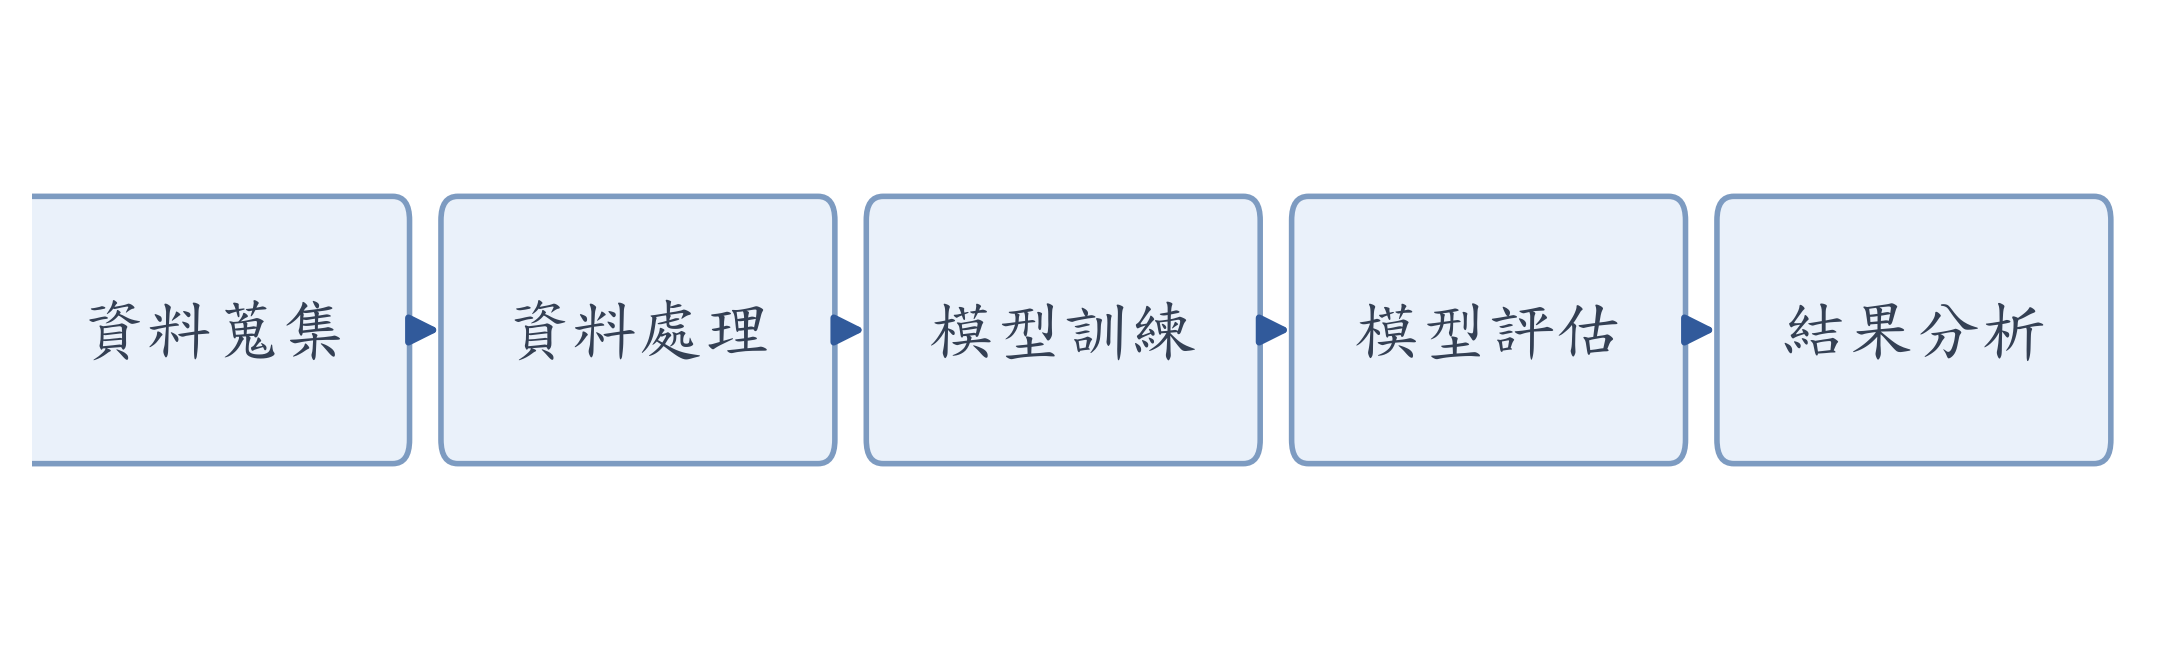
\includegraphics[width=0.6\linewidth,height=5cm,keepaspectratio]{figures/samples/architecture.png}
  \caption{Description}
  \label{fig:custom}
\end{figure}
\end{lstlisting}

\code{width} sets the displayed width; \code{0.6\linewidth} is sixty percent of the available text width, and a fixed length such as \code{8cm} also works. \code{height} sets the displayed height and, when omitted, follows the original proportions. Giving both stretches the image out of shape unless you add \code{keepaspectratio}, in which case the whole image keeps its proportions and is scaled to fit inside that area.

Other common options are \code{page} (which page of a multi-page PDF to insert, \code{1} by default) and \code{trim} with \code{clip} (cropping the edges). For the full list of parameters see the \href{https://ctan.org/pkg/graphicx}{documentation of graphicx}. A figure written the standard way does not follow \code{layout.caption-position.image}; to put its caption above, write \code{\caption} before \code{\includegraphics}.

\section{Side-by-side Figures}

To put two figures on the same row, use the \code{figrow} environment and give the path and sub-caption of each figure in order. The sub-captions are numbered \code{(a)}, \code{(b)} and so on automatically, and the whole group shares one figure number and one overall caption, so the list of figures shows only one entry. Here is how two figures are written:

\begin{lstlisting}[language=latex]
\begin{figrow}{Function graph comparison}{fig:row}
  \subfig{figures/samples/sin-x.pdf}{$\sin x$}
  \subfig{figures/samples/x-sin-x.pdf}{$x \sin x$}
\end{figrow}
\end{lstlisting}

\begin{figrow}{Function graph comparison}{fig:row}
  \subfig{figures/samples/sin-x.pdf}{$\sin x$}
  \subfig{figures/samples/x-sin-x.pdf}{$x \sin x$}
\end{figrow}

If you do not need sub-captions, leave the second brace empty. If the figures sit too close together after compiling, add \code{[gutter=2em]} after the environment name to widen the gap between the two columns, then check that the figures still have enough room.

\begin{lstlisting}[language=latex]
\begin{figrow}[gutter=2em]{Function graph comparison}{}
  \subfig{figures/samples/sin-x.pdf}{}
  \subfig{figures/samples/x-sin-x.pdf}{}
\end{figrow}
\end{lstlisting}

The \code{width} of side-by-side figures is relative to the width of each one's own column: with \code{[width=0.8]}, every figure takes eighty percent of its column. This is the value to lower when a figure needs to shrink; you need not edit the original image first.

\section{Grid Figures}

If there are more figures and you want several rows, use \code{figgrid} instead. \code{rows} sets the number of rows and \code{columns} the number of columns per row. The four figures below are placed with \code{rows=2} and \code{columns=2}, which lays them out in two rows from left to right and top to bottom. The sub-caption of each figure and the overall caption of the group are written just as for side-by-side figures.

\begin{lstlisting}[language=latex]
\begin{figgrid}[rows=2,columns=2,placement=auto]{Model predictions}{fig:grid}
  \subfig{figures/samples/a.pdf}{Linear model}
  \subfig{figures/samples/b.pdf}{Decision tree}
  \subfig{figures/samples/c.pdf}{Random forest}
  \subfig{figures/samples/d.pdf}{Neural network}
\end{figgrid}
\end{lstlisting}

\begin{figgrid}[rows=2,columns=2,placement=auto]{Model predictions}{fig:grid}
  \subfig{figures/samples/a.pdf}{Linear model}
  \subfig{figures/samples/b.pdf}{Decision tree}
  \subfig{figures/samples/c.pdf}{Random forest}
  \subfig{figures/samples/d.pdf}{Neural network}
\end{figgrid}

The four figures use the same synthetic training data: open circles are observed values, and solid black lines are each model's predictions. The data serve only to demonstrate the layout and are not experimental results of a real thesis. \code{placement=auto} lets \LaTeX{} treat the group as an ordinary float and decide, from the space left on the page, whether it stays in place or moves to a suitable position; when omitted it is \code{placement=none} and the group stays where it is written. \code{figrow} and \code{\fig} accept the same option, for example \code{\fig[width=0.6\linewidth,placement=auto]\{...\}}.

For two rows of three, set \code{rows=2,columns=3}. The figures are rearranged in the order they are given; the example below adds K-nearest neighbours and support vector regression after the first four models, filling all six cells. \code{rows} can be left out so that the number of rows grows with the number of figures; if you do specify a row count, the number of figures cannot exceed \code{rows * columns}. After adjusting, check that the text inside the figures is still legible; if it has become too small, reduce the number of columns.

\begin{lstlisting}[language=latex]
\begin{figgrid}[rows=2,columns=3]{Two rows, three columns}{fig:grid-2x3}
  \subfig{figures/samples/a.pdf}{Linear model}
  \subfig{figures/samples/b.pdf}{Decision tree}
  \subfig{figures/samples/c.pdf}{Random forest}
  \subfig{figures/samples/d.pdf}{Neural network}
  \subfig{figures/samples/e.pdf}{K-nearest neighbours}
  \subfig{figures/samples/f.pdf}{Support vector regression}
\end{figgrid}
\end{lstlisting}

The result is shown in \figref{fig:grid-2x3}:

\begin{figgrid}[rows=2,columns=3]{Two rows, three columns}{fig:grid-2x3}
  \subfig{figures/samples/a.pdf}{Linear model}
  \subfig{figures/samples/b.pdf}{Decision tree}
  \subfig{figures/samples/c.pdf}{Random forest}
  \subfig{figures/samples/d.pdf}{Neural network}
  \subfig{figures/samples/e.pdf}{K-nearest neighbours}
  \subfig{figures/samples/f.pdf}{Support vector regression}
\end{figgrid}

\section{Tables}

There are two ways to write a table: use the \code{tbl} environment when you need a rule around every cell, and the template's \code{tlt} environment for a three-line table, which has only the rules above and below the header and under the last row. The data are filled in the same way in both; only the look and the rules differ, so pick one according to your thesis or department rules.

\subsection{Traditional Tables}

When every cell needs a border, use the \code{tbl} environment. Its parameters are the caption, the label and the column format, and the column format works as in \code{tabular}: \code{ccc} means three centred columns, and adding \code{|} between columns draws vertical lines. Fill in the data from left to right and top to bottom, separate cells with \code{&}, end a row with \code{\\}, and draw a horizontal line with \code{\hline}.

\begin{lstlisting}[language=latex]
\begin{tbl}{Results (traditional table)}{tbl:traditional}{|c|c|c|}
  \hline
  Batch size & Accuracy (\%) & Training time (s) \\
  \hline
  32  & 91.2 & 48 \\
  64  & 92.8 & 31 \\
  128 & 92.1 & 22 \\
  \hline
\end{tbl}
\end{lstlisting}

\begin{tbl}{Results (traditional table)}{tbl:traditional}{|c|c|c|}
  \hline
  Batch size & Accuracy (\%) & Training time (s) \\
  \hline
  32  & 91.2 & 48 \\
  64  & 92.8 & 31 \\
  128 & 92.1 & 22 \\
  \hline
\end{tbl}

Adjacent cells can be merged. \code{\multicolumn{2}{c}{text}} lets one cell span two columns; in the three-column table below the ``Total'' row has only two cells, because ``100 samples'' already takes up the last two columns and there is no need to add a third. For a cell that spans two rows, use \code{\multirow{2}{*}{text}}; leave the occupied position in the next row empty.

\begin{lstlisting}[language=latex]
\begin{tbl}{Merged cells}{tbl:merged}{|c|c|c|}
  \hline
  Item & Training set & Test set \\
  \hline
  Samples & 80 & 20 \\
  \hline
  Total & \multicolumn{2}{c|}{100 samples} \\
  \hline
\end{tbl}
\end{lstlisting}

\begin{tbl}{Merged cells}{tbl:merged}{|c|c|c|}
  \hline
  Item & Training set & Test set \\
  \hline
  Samples & 80 & 20 \\
  \hline
  Total & \multicolumn{2}{c|}{100 samples} \\
  \hline
\end{tbl}

\subsection{Three-line Tables}

Unlike the traditional table that puts a border on every cell, the three-line table comes from the table conventions of \href{https://apastyle.apa.org/style-grammar-guidelines/tables-figures/tables}{APA style} and is most common in fields with many statistics, such as social science, education and psychology. Without the many vertical and horizontal lines the page looks cleaner, which is especially easy to read when whole columns are numbers. Most of the official regulations collected in \code{docs/} do not say which kind of rules a table should use; which one applies is usually the academic habit of the department or advisor rather than a school-wide rule, so it is worth confirming before you write.

A three-line table keeps only three horizontal rules: above and below the header and at the foot. With \code{tlt}, the top and bottom rules are drawn by the environment, and you write a \code{\midrule} yourself for the rule under the header. The data from before are reused below to make comparison easy.

\begin{lstlisting}[language=latex]
\begin{tlt}[notes={The values are layout samples.}]{Summary of results}{tbl:batch}{ccc}
  Batch size & Accuracy (\%) & Training time (s) \\
  \midrule
  32  & 91.2 & 48 \\
  64  & 92.8 & 31 \\
  128 & 92.1 & 22 \\
\end{tlt}
\end{lstlisting}

\begin{tlt}[notes={The values are layout samples.}]{Summary of results}{tbl:batch}{ccc}
  Batch size & Accuracy (\%) & Training time (s) \\
  \midrule
  32  & 91.2 & 48 \\
  64  & 92.8 & 31 \\
  128 & 92.1 & 22 \\
\end{tlt}

After the data are in, you can adjust column widths, alignment and the note under the table. The options in square brackets and the three arguments after them are:

\begin{tlt}{Common parameters of the three-line table}{tbl:tlt-args}{L{0.2\linewidth}L{0.7\linewidth}}
Parameter & Purpose and example \\
\midrule
Column format & \code{l}, \code{c}, \code{r} size by content; \code{L{4cm}} is a fixed-width left-aligned column, for longer text. \\
\code{width} & Option. Given a total width (e.g. \code{width=\linewidth}), the column format may use \code{X} to share the remaining width; when cells contain \code{\code}, use \code{L{...}} instead. \\
\code{thick}, \code{thin} & Options. Weight of the top and bottom rules and of the rule under the header; pass them to change one table only, or edit \code{\heavyrulewidth} at the top of the table section of \code{tw-thesis.sty} to change all tables. \\
\code{notes} & Option. A note under the table, at ninety percent of the body size. \\
\code{notes-label} & Option. The prefix of the note; ``Note.'' by default, and an empty \code{{}} removes it. \\
\end{tlt}

If there is so much data that a table does not fit on one page, \code{tlt} and \code{tbl} do not break across pages; use the \code{longtable} environment instead and add \code{\toprule}, \code{\midrule} and \code{\bottomrule} yourself; its \code{\endhead} repeats the header on every page. Afterwards check where the pages break and make sure readers can still tell the columns apart.

Three-line tables can merge cells too: in the example below, the ``Total'' row fills only two cells yet still occupies all three columns; compared with the traditional table above, the only difference is the style of the rules.

\begin{lstlisting}[language=latex]
\begin{tlt}{Merged cells in a three-line table}{tbl:tlt-merged}{ccc}
  Item & Training set & Test set \\
  \midrule
  Samples & 80 & 20 \\
  Total & \multicolumn{2}{c}{100 samples} \\
\end{tlt}
\end{lstlisting}

\begin{tlt}{Merged cells in a three-line table}{tbl:tlt-merged}{ccc}
  Item & Training set & Test set \\
  \midrule
  Samples & 80 & 20 \\
  Total & \multicolumn{2}{c}{100 samples} \\
\end{tlt}

The header itself can be grouped and set in two rows. When several columns fall into one category (for example ``Training set'' and ``Test set'' each split into accuracy and loss), split the header into two rows: the first uses \code{\multicolumn{2}{c}{...}} to span several columns and give the group name, and the second supplies the real name of each column; columns that need no grouping (such as ``Model'' on the far left) use \code{\multirow{2}{*}{...}} to span both header rows so no blank is left. To put a short rule under each group name, mark the range with \code{\cmidrule(lr){a-b}}, a command from the \code{booktabs} package, where \code{(lr)} leaves a little gap between the two short rules. To add a note to a single cell, put a superscript letter such as \code{\textsuperscript{a}} after its content and explain it in \code{notes}:

\begin{lstlisting}[language=latex]
\begin{tlt}[notes={\textsuperscript{a} Training stopped early (early stopping) and did not run the full number of epochs.}]{Grouped header}{tbl:tlt-grouped}{ccccc}
  \multirow{2}{*}{Model} & \multicolumn{2}{c}{Training set} & \multicolumn{2}{c}{Test set} \\
  \cmidrule(lr){2-3} \cmidrule(lr){4-5}
  & Accuracy (\%) & Loss & Accuracy (\%) & Loss \\
  \midrule
  Linear model & 88.1 & 0.42 & 85.3 & 0.51 \\
  Random forest & 96.4\textsuperscript{a} & 0.11 & 90.2 & 0.28 \\
\end{tlt}
\end{lstlisting}

\begin{tlt}[notes={\textsuperscript{a} Training stopped early (early stopping) and did not run the full number of epochs.}]{Grouped header}{tbl:tlt-grouped}{ccccc}
  \multirow{2}{*}{Model} & \multicolumn{2}{c}{Training set} & \multicolumn{2}{c}{Test set} \\
  \cmidrule(lr){2-3} \cmidrule(lr){4-5}
  & Accuracy (\%) & Loss & Accuracy (\%) & Loss \\
  \midrule
  Linear model & 88.1 & 0.42 & 85.3 & 0.51 \\
  Random forest & 96.4\textsuperscript{a} & 0.11 & 90.2 & 0.28 \\
\end{tlt}

In every row, the number of cells plus the columns each \code{\multicolumn} occupies must equal the number of columns in the column format: the first row is \code{1 + 2 + 2 = 5}, and the second leaves the first cell empty and fills four more; otherwise the table is laid out wrongly.

The three rules that \code{tlt} draws all come from the \code{booktabs} package and can be used directly inside a table:

\begin{tlt}{Rule commands of the three-line table}{tbl:booktabs}{L{0.3\linewidth}L{0.55\linewidth}}
Command & Where the rule goes \\
\midrule
\code{\toprule} & Top of the table; \code{tlt} draws it automatically \\
\code{\midrule} & Below the header, or between blocks \\
\code{\bottomrule} & Bottom of the table; \code{tlt} draws it automatically \\
\code{\cmidrule{a-b}} & Only over columns \code{a} to \code{b} (inclusive) \\
\end{tlt}

With \code{tlt}, only the \code{\midrule} below the header needs writing yourself; to add another rule in the middle of the data (for example to split it into two blocks of subtotals), just write one more \code{\midrule}. If you do not want \code{tlt} at all, you can also use the \code{tbl} environment and build the booktabs look yourself. For example:

\begin{lstlisting}[language=latex]
\begin{tbl}{Hand-built table with booktabs rules}{}{ccc}
  \toprule
  Item & Group 1 & Group 2 \\
  \midrule
  Mean & 91.2 & 88.5 \\
  Std. dev. & 3.1 & 4.2 \\
  \midrule
  Samples & \multicolumn{2}{c}{60} \\
  \bottomrule
\end{tbl}
\end{lstlisting}

The two numbers in \code{\cmidrule{a-b}} are column numbers counted from 1 and inclusive; for example the \code{\cmidrule(lr){2-3}} in the grouped-header example above means columns 2 to 3. The default rule weights are \code{0.08em} for \code{\toprule} and \code{\bottomrule} and \code{0.05em} for \code{\midrule} and \code{\cmidrule}.

The three rules of \code{tlt} can be made thicker too. To change only one table, pass the \code{thick} and \code{thin} options:

\begin{lstlisting}[language=latex]
\begin{tlt}[thick=0.14em]{Thicker top and bottom rules}{tbl:thick}{cc}
  Item & Value \\
  \midrule
  Example & 1 \\
\end{tlt}
\end{lstlisting}

\begin{tlt}[thick=0.14em]{Thicker top and bottom rules}{tbl:thick}{cc}
  Item & Value \\
  \midrule
  Example & 1 \\
\end{tlt}

Compare the top and bottom rules of \tblref{tbl:batch} to see the difference \code{thick} makes. To give all tables the same weight (including those built by hand with \code{\toprule}, \code{\midrule}, \code{\bottomrule} and \code{\cmidrule}), edit the lengths at the top of the table section of \code{tw-thesis.sty}:

\begin{lstlisting}[language=latex]
\setlength\heavyrulewidth{0.08em}   % \toprule, \bottomrule
\setlength\lightrulewidth{0.05em}   % \midrule, \cmidrule
\setlength\cmidrulewidth{0.05em}
\end{lstlisting}

\section{Cross-references}

To mention a figure or table in the text, first give it a label and then refer to it with \code{\ref}. Labels can be named freely, but must not repeat within the document. The earlier examples already carry \code{fig:grid} and \code{tbl:batch}, so you can use the following directly:

\begin{lstlisting}[language=latex]
The four sample figures are arranged as shown in \figref{fig:grid}.
See \tblref{tbl:batch} for the detailed numbers.
This chapter follows the rules of \ref{cha:layout}.
\end{lstlisting}

After compiling, the labels turn into the matching numbers: the four sample figures are arranged as shown in \figref{fig:grid}, see \tblref{tbl:batch} for the numbers, and this chapter follows the rules of \ref{cha:layout}. Section references show the full hierarchy, so \ref{sec:caption} shows the chapter and section numbers. All of these references are clickable and jump to the figure, table or section.

\code{\figref}, \code{\tblref} and \code{\lstref} put ``Figure'', ``Table'' and ``Listing'' in front of the number; the word comes from \code{strings:}. If you want only the number, use \code{\ref}. After figures or tables are added or moved, the template renumbers them and the references in the text follow, so you never edit ``Figure n'' or ``Table n'' by hand. Section headings can be referred to the same way; just add a label after the heading:

\begin{lstlisting}[language=latex]
\chapter{Layout Settings}\label{cha:layout}
\section{Margins and Paper}\label{sec:margin}
\end{lstlisting}

The wording of section references is set under \code{cross-ref:} in \code{config.yml}. \code{C} is the chapter number, \code{S} the section number and \code{B} the subsection number; only the numbers needed at the level of the label are shown. The default uses Chinese numerals and shows ``第C章'', ``第C章第S節'' or ``第C章第S節第B小節'' by level. To show \code{2}, \code{2.5} and \code{2.5.1} instead, change it to:

\begin{lstlisting}[language=yaml]
cross-ref:
  numbering: "1"
  chapter: "C"
  section: "C.S"
  subsection: "C.S.B"
\end{lstlisting}

To add words, use \code{{C}}, \code{{S}} and \code{{B}}, for example \code{"Ch. {C} Sec. {S}"}. The style affects only the section references in the text; it does not change headings, the table of contents, figures, tables, citations or page references, and appendices keep labels such as ``Appendix A''.

A Chinese character can follow a reference directly: write \code{see\ref{sec:caption}} and \LaTeX{} adds no extra space between them. Around punctuation, leave spaces as the sentence needs.

To put your own words in front of a reference, do not use \code{\figref}; write \code{Table~\ref{tbl:batch}} directly. This is a per-reference approach and changes only that one spot. If the prefix of ``Figure 1'' and ``Table 1'' in captions and in the lists also needs to change, start from the source, which is the \code{strings:} described in a later section, instead of rewriting each reference.

\section{Math and the List of Symbols}

To put a formula in a sentence, wrap it in \code{$...$}, for example \code{$E = m c^2$}. To display it on its own line, use \code{\[ ... \]}; to number it, use the \code{equation} environment instead. This is \LaTeX{}'s native math syntax; see the \href{https://ctan.org/pkg/amsmath}{documentation of amsmath} for the full set of symbols. The template already loads \code{amsmath} and \code{amssymb}.

\begin{lstlisting}[language=latex]
Inline formula $E = m c^2$, and a display formula:

\[
  \int_0^1 x^2 \,\mathrm{d}x = \frac{1}{3}
\]
\end{lstlisting}

After compiling, the inline formula $E = m c^2$ sits in the same paragraph as the text and the integral below stands on its own line:

\[ \int_0^1 x^2 \,\mathrm{d}x = \frac{1}{3} \]

To refer to a formula later, use an \code{equation} environment and add a label after the formula. The example below uses \code{eq:pythagoras} as the name, and referring works as for figures and tables; \code{\eqref} prints the parentheses as well:

\begin{lstlisting}[language=latex]
\begin{equation}\label{eq:pythagoras}
  a^2 + b^2 = c^2
\end{equation}

As shown in \eqref{eq:pythagoras}.
\end{lstlisting}

\begin{equation}\label{eq:pythagoras}
  a^2 + b^2 = c^2
\end{equation}

As shown in \eqref{eq:pythagoras}. The numbering rule of formulas is set by \code{config.yml}, so you never write \code{(1)} by hand; by default every formula is numbered continuously as \code{(1)}, \code{(2)}...; if your department wants numbering by chapter (for example formulas in Chapter 3 shown as \code{(3.1)}, \code{(3.2)}, restarting from \code{(4.1)} in Chapter 4), set this under \code{layout:} in \code{config.yml}:

\begin{lstlisting}[language=yaml]
layout:
  equation-numbering: "1"      # 1 | a | A | i | I | *
  equation-per-chapter: true   # true numbers as "chapter.count" and restarts every chapter
\end{lstlisting}

\code{equation-numbering} decides only the style of the running number and is written like \code{footnote-numbering}; the chapter number is always Arabic and does not depend on this setting.

If the thesis uses abbreviations or mathematical symbols repeatedly, collect them in the list of symbols among the front pages. Open \code{contents/front/denotation.tex}, keep the \code{denotation} environment, and fill in entries with the syntax below. Each entry starts with \code{\item}, with the symbol in square brackets and the full name or definition after it:

\begin{lstlisting}[language=latex]
\begin{description}
  \item[CNN] Convolutional Neural Network
  \item[$\eta$] learning rate
\end{description}
\end{lstlisting}

\section{Figure and Table Captions}

The words ``Figure'' and ``Table'' (圖 and 表 in a Chinese thesis) appear in captions, in the lists of figures and tables and in every reference in the text; they are set in one place, under \code{strings:} in \code{config.yml}, so you never change them one by one:

\begin{lstlisting}[language=yaml]
strings:
  figure: "插圖" # figure prefix of a Chinese thesis, "圖" by default
  figure-en: "Fig." # used when language: english, "Figure" by default
  table: "附表" # table prefix of a Chinese thesis, "表" by default
  table-en: "Tab." # used when language: english, "Table" by default
\end{lstlisting}

After changing them, recompile and every figure and table produced by \code{\fig}, \code{figrow}, \code{figgrid}, \code{tlt} and \code{tbl} takes the new prefix, and the lists of figures and tables and the text of \code{\figref} and \code{\tblref} follow. If only one figure or table needs to differ from the rest, use the standard \code{figure} environment and write the name you want yourself:

\begin{lstlisting}[language=latex]
\begin{figure}[htbp]
  \centering
  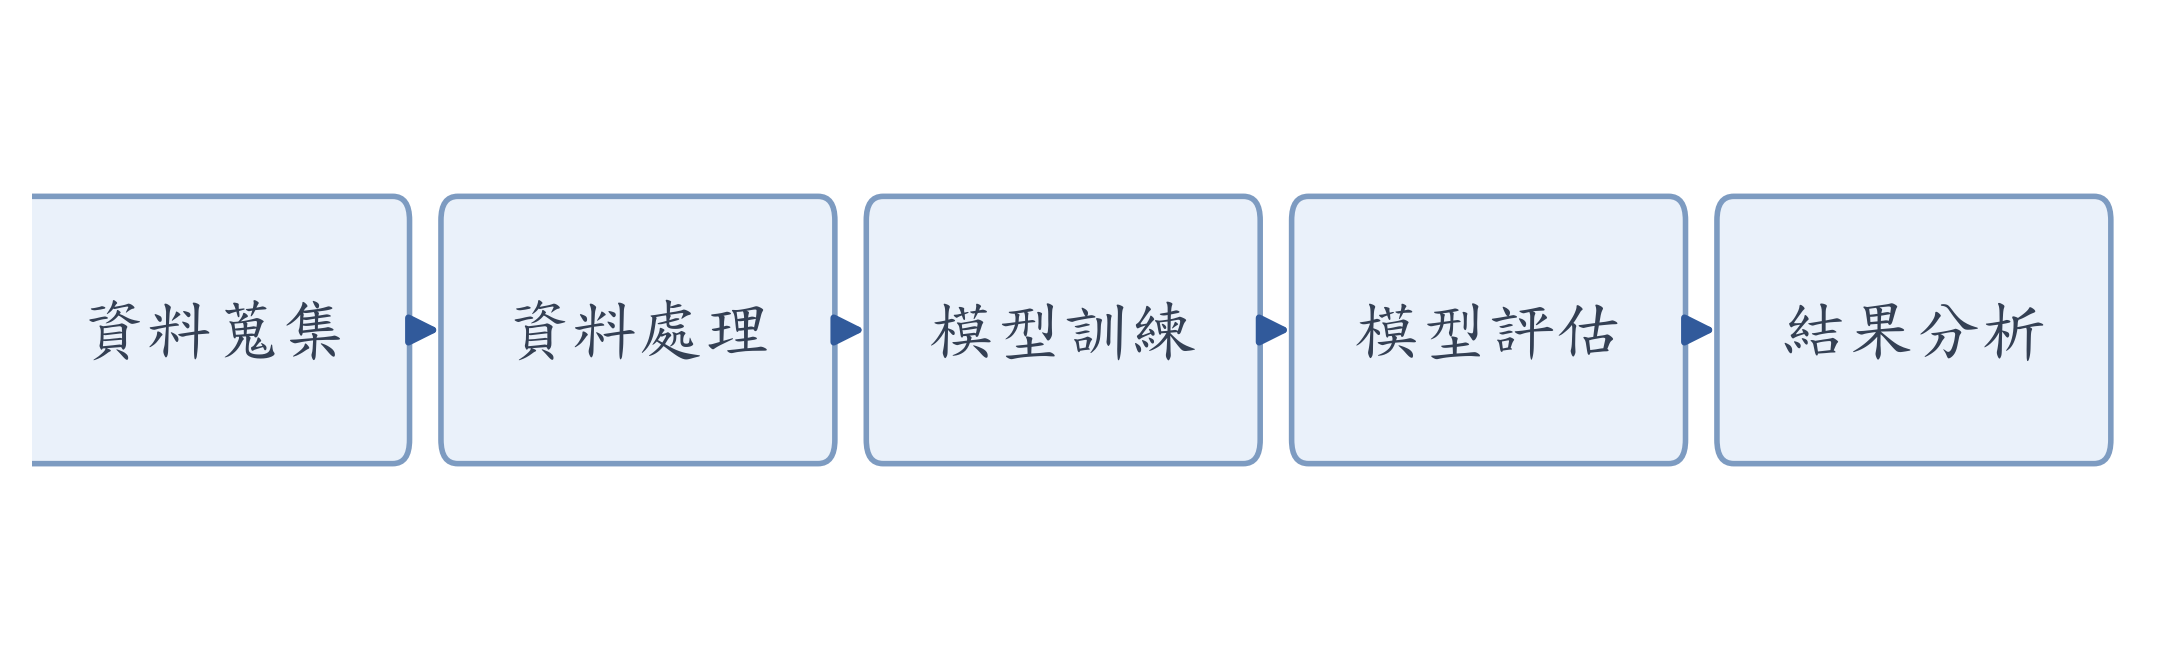
\includegraphics[width=0.6\linewidth]{figures/samples/architecture.png}
  \caption{Description}\label{fig:special}
\end{figure}
\end{lstlisting}

To make a figure show only its number without the prefix text, use \code{\caption*} for no numbering, or adjust \code{\captionsetup} of the \code{caption} package yourself; see the \href{https://ctan.org/pkg/caption}{documentation of caption}.

\section{Footnotes}

For additional remarks on figures and tables, the grouped-header example earlier put \code{\textsuperscript{a}} in a cell and explained it in \code{notes}; but that is a hand-made superscript, not a real footnote. For notes you can drop in anywhere in the text, numbered and typeset automatically by \LaTeX{}, use \code{\footnote{...}}; no other file needs editing, and the number, the superscript and the rule at the foot of the page are all handled for you:

\begin{lstlisting}[language=latex]
This point is somewhat disputed\footnote{Studies disagree on it.}, and later chapters return to it.
\end{lstlisting}

The result:

This point is somewhat disputed\footnote{Studies disagree on it.}, and later chapters return to it.

At the bottom of the page, numbering starts at 1 and keeps counting through the whole text, without resetting at page breaks. To cite the same note in several places, give a label to the first \code{\footnote}; you can then reuse the same number with \code{\footref} without creating a new footnote:

\begin{lstlisting}[language=latex]
First mention\footnote{The note text.}\label{fn:first}, and the second time\footref{fn:first}.
\end{lstlisting}

The number format and whether numbering restarts every chapter are both set under \code{layout:} in \code{config.yml}:

\begin{lstlisting}[language=yaml]
layout:
  footnote-numbering: "1"      # 1 | a | A | i | I | *
  footnote-per-chapter: false  # true restarts from 1 in each chapter
\end{lstlisting}

\code{footnote-numbering} is written like \code{outline.body-numbering} and the other numbering settings: \code{"1"} is Arabic numerals, \code{"a"} and \code{"A"} are letters, \code{"i"} and \code{"I"} are lower and upper case Roman numerals, and \code{"*"} is a star, then two stars and so on, which suits a thesis with few footnotes. \code{footnote-per-chapter} is \code{false} by default, so numbering runs on through the whole text; if your department wants each chapter to restart from 1, change it to \code{true}, with no need to reset the counter by hand at the start of every chapter.

With figures, tables, footnotes and formulas covered, the next chapter explains citing the literature, and code and appendices.

\chapter{References, Code and Appendices}\label{cha:refs}

This chapter continues with citing the literature, code, and appendices. The examples of the sections do not depend on one another; copy whichever you need and replace it with your own thesis data.

The files for the references and appendices live in \code{contents/back/}, and the other examples can be written straight into this chapter. When moving or editing content, remember to update the matching lines in \code{main.tex} at the same time, so that the order of the references or appendices does not slip.

\section{Citing the Literature}

A \code{.bib} file is a plain-text bibliography database in \BibTeX{} format; one entry corresponds to one work, in the form \code{@type{key, field = {value}, ...}}. \code{contents/back/references.bib} already holds a few sample entries, one of which looks like this:

\begin{lstlisting}
@inproceedings{kocher99,
  author =       {C. Kocher and J. Jaffe and B. Jun},
  title =        {Differential Power Analysis},
  editor =       {M. Wiener},
  booktitle =    {Advances in Cryptology ({CRYPTO}~'99)},
  series =       {Lecture Notes in Computer Science},
  volume =       1666,
  pages =        {388-397},
  publisher =    {Springer-Verlag},
  month =        {August},
  year =         1999
}
\end{lstlisting}

\code{@inproceedings} is the entry type (a conference paper); others you will often see are \code{@article} (journal article), \code{@book} and \code{@incollection} (a chapter in a book), and the type affects which fields the reference list shows. \code{kocher99} is the key used to cite the entry in the text and must not repeat within one \code{.bib}; the \code{author}, \code{title}, \code{year} and other fields that follow are the data of the work, filled in one by one, and their order does not affect the result.

Below each search result, Google Scholar has a ``Cite'' button, and at the bottom of its pop-up window is a \BibTeX{} link that copies the whole entry; the pages of library databases (such as IEEE Xplore and the ACM Digital Library) mostly have an ``Export Citation'' or ``Cite'' function too, where you choose the \BibTeX{} format. If you usually work with a reference manager such as Zotero or EndNote, you can also export a \code{.bib} file directly. Once you have an entry, paste it into \code{references.bib}, change the key to a name you can remember (for example \code{surname+year}), and check that it does not repeat an existing entry.

With the data ready, go back to the chapter file and cite with the same key. To put a work at the end of a sentence, use \code{\citep}; to put the author into the sentence, use \code{\citet}. The forms that show only the author or the year are listed too, so choose whichever the sentence needs. These four commands come from the \code{citation-style-language} package, which the template already loads.

\begin{lstlisting}[language=latex]
\citep{kocher99}       % parenthetical citation
\citet{kocher99}       % in-text citation
\citeauthor{kocher99}  % author only
\citeyear{kocher99}    % year only
\end{lstlisting}

The differences among the four commands after compiling are as follows; check them first and then replace the key with the work you want to cite:

\begin{tlt}{Comparison of citation commands}{tbl:cite-forms}{L{0.3\linewidth}L{0.25\linewidth}L{0.35\linewidth}}
Command & Result & Use \\
\midrule
\code{\citep{kocher99}} & \citep{kocher99} & Parenthetical, at the end of a sentence \\
\code{\citet{kocher99}} & \citet{kocher99} & In-text, the author is part of the sentence \\
\code{\citeauthor{kocher99}} & \citeauthor{kocher99} & Shows only the author \\
\code{\citeyear{kocher99}} & \citeyear{kocher99} & Shows only the year \\
\end{tlt}

To cite a particular passage in a book, add a page or chapter in square brackets. The example below uses the entry \code{companion} and adds ``page 42''; when you apply it to your own thesis, change it to the location you actually cite:

\begin{lstlisting}[language=latex]
\citep[p.~42]{companion}
\end{lstlisting}

After compiling it appears as \citep[p.~42]{companion}. The page is typeset together with the citation, and the punctuation and arrangement are decided by the reference style you chose.

To cite several works at once, separate the keys with commas, for example \code{\citep{kocher99,IEEE-1363}}. Like a single citation, it uses the reference style from the config, so pick whichever way you are more used to.

\section{Reference Settings}

Open \code{config.yml} and add the settings you need under the existing \code{bibliography:} block. \code{path} names the bibliography files and \code{style} decides the citation format; if your data are spread over several files, list the paths in \code{path} in order.

\begin{lstlisting}[language=yaml]
bibliography:
  path: ["/contents/back/references.bib"] # several files allowed
  style: "apa"       # built-in CSL style name, or the path of a .csl file; see the table below
  title: "參~考~文~獻"
  color: "#0000ff"   # colour of citations and links; use "#000000" for black-and-white print
  full: false        # true also lists entries that were not cited
\end{lstlisting}

\code{path} may mix \code{.bib}, Hayagriva \code{.yml} (the format of the Typst version) and CSL JSON/YAML; Hayagriva files are converted to CSL JSON automatically when \code{scripts/gen.lua} runs, so you need not convert them yourself. A citation key cannot appear in two different files.

\code{style} decides the logic of the references and falls roughly into three systems: author-date shows the author's name and year in the text, so readers see at a glance how old the study is; author-page shows the author and page, which makes it easy to check the source; and numeric keeps only a number or superscript in the text and orders the list by number, the least distracting to read. Those in common use in each field are:

\begin{tlt}[notes={\texttt{mla} is short for \texttt{modern-language-association}; either spelling works.}]{Common reference formats}{tbl:citation-styles}{L{0.12\linewidth}L{0.17\linewidth}L{0.25\linewidth}L{0.26\linewidth}}
Format & System & Typical field & \code{style} value \\
\midrule
APA & Author-date & Psychology, education, social science & \code{apa} \\
Harvard & Author-date & Business, social science & \code{harvard-cite-them-right} \\
Chicago & Author-date & History, humanities & \code{chicago-author-date} \\
MLA & Author-page & Literature, languages, arts & \code{mla} \\
IEEE & Numeric & Computer science, electrical engineering & \code{ieee} \\
Vancouver & Numeric & Medicine, nursing & \code{vancouver} \\
\end{tlt}

Just change \code{style} to the value in the last column of the table, for example \code{"apa"} to \code{"ieee"}, and after recompiling the citations in the text and the list at the end switch to the matching style together, with no need to change how \code{\citep}, \code{\citet} and the others are written. After changing it, look at both the body and the reference page to check how the authors, years or numbers are shown.

The list above shows only the most common ones, and many more styles are available; if the format your department names is not among them, obtain the matching \code{.csl} style file (Bluebook, commonly used in law, is one example) and give its path in \code{style}, for example \code{style: "/misc/my-style.csl"}.

The default \code{full: false} lists only the works cited in the text. If a new entry still does not appear in the list, first check that the text cites it and that the capitalisation of its key matches. To list every entry of the bibliography file for the time being, change it to \code{true} and check the data entry by entry.

The place where the references are inserted is decided by \code{\references} in \code{main.tex}. Below it sits after Chapter 4 and before the appendices; if your department wants a different binding order, just move this line, with no need to copy the reference list by hand:

\begin{lstlisting}[language=latex]
\chapter{文獻、程式碼與附錄}\label{cha:refs}

本章接續說明文獻引用、程式碼與附錄的寫法。各節範例互不依賴，需要哪個就照抄哪段，再換成自己論文的資料即可。

文獻與附錄的檔案放在 \code{contents/back/}，其餘範例可以直接寫進本章。搬動或修改內容時，記得同步更新 \code{main.tex} 裡對應的引用位置，以免參考文獻或附錄的順序跑掉。

\section{引用文獻}

\code{.bib} 是以 \BibTeX{} 格式儲存的純文字文獻資料庫，一筆文獻對應一個條目，格式是 \code{@類型{識別名稱, 欄位 = {值}, ...}}。\code{contents/back/references.bib} 已經收錄幾筆範例，其中一筆長這樣：

\begin{lstlisting}
@inproceedings{kocher99,
  author =       {C. Kocher and J. Jaffe and B. Jun},
  title =        {Differential Power Analysis},
  editor =       {M. Wiener},
  booktitle =    {Advances in Cryptology ({CRYPTO}~'99)},
  series =       {Lecture Notes in Computer Science},
  volume =       1666,
  pages =        {388-397},
  publisher =    {Springer-Verlag},
  month =        {August},
  year =         1999
}
\end{lstlisting}

\code{@inproceedings} 是文獻類型（研討會論文），常見的還有 \code{@article}（期刊論文）、\code{@book}（書籍）、\code{@incollection}（專書篇章）等，類型會影響參考文獻頁該顯示哪些欄位。\code{kocher99} 是識別名稱，用來在內文引用這筆文獻，同一份 \code{.bib} 裡不能重複；後面的 \code{author}、\code{title}、\code{year} 等則是這筆文獻的資料，逐欄填入即可，順序不影響排版結果。

Google Scholar 每筆搜尋結果下方的「引用」按鈕，彈出視窗最下面就有 \BibTeX{} 連結，點開即可複製整個條目；圖書館資料庫（如 IEEE Xplore、ACM Digital Library）的文獻頁面也大多有「Export Citation」或「Cite」功能，選 \BibTeX{} 格式匯出。若平常使用 Zotero、EndNote 等文獻管理軟體，同樣可以直接匯出 \code{.bib} 檔。拿到條目後貼進 \code{references.bib}，把識別名稱改成自己好記的名字（例如 \code{作者姓+年份}），再確認沒有跟既有條目重複即可。

文獻資料準備好後，回到章節檔案，使用相同的識別名稱引用。若要把文獻放在句尾，可以使用 \code{\citep}；若要把作者寫進句子，則使用 \code{\citet}。以下也列出只顯示作者或年份的寫法，可以依句子需要選用。這四個指令來自 \code{citation-style-language} 套件，模板已經載入。

\begin{lstlisting}[language=latex]
\citep{kocher99}       % 括號引用
\citet{kocher99}       % 行文引用
\citeauthor{kocher99}  % 只要作者
\citeyear{kocher99}    % 只要年份
\end{lstlisting}

四個指令編譯後的差異如下，請先對照確認，再將識別名稱換成自己要引用的文獻：

\begin{tlt}{文獻引用指令對照}{tbl:cite-forms}{L{0.3\linewidth}L{0.25\linewidth}L{0.35\linewidth}}
指令 & 顯示結果 & 用途 \\
\midrule
\code{\citep{kocher99}} & \citep{kocher99} & 括號引用，放在句尾 \\
\code{\citet{kocher99}} & \citet{kocher99} & 行文引用，把作者寫進句子 \\
\code{\citeauthor{kocher99}} & \citeauthor{kocher99} & 只顯示作者 \\
\code{\citeyear{kocher99}} & \citeyear{kocher99} & 只顯示年份 \\
\end{tlt}

引用書中的特定段落時，可以用方括號補上頁碼或章節。以下以 \code{companion} 這筆文獻為例，加入「第 42 頁」；套用到自己的論文時，請改成實際引用的位置：

\begin{lstlisting}[language=latex]
\citep[第 42 頁]{companion}
\end{lstlisting}

編譯後會顯示為 \citep[第 42 頁]{companion}。頁碼會與文獻引用一起排版，標點和排列方式則由選用的參考文獻樣式決定。

若要一次引用多筆，把識別名稱用逗號隔開，例如 \code{\citep{kocher99,IEEE-1363}}。這種寫法與單筆引用一樣會使用設定檔中的文獻樣式，可以選擇自己較習慣的方式。

\section{參考文獻設定}

請打開 \code{config.yml}，在既有的 \code{bibliography:} 區塊下加入需要的設定。\code{path} 用來指定文獻檔案，\code{style} 決定引用格式；若資料分散在多個檔案，可以在 \code{path} 的清單中依序加入路徑。

\begin{lstlisting}[language=yaml]
bibliography:
  path: ["/contents/back/references.bib"] # 可以給多個檔案
  style: "apa"       # 內建 CSL 樣式名稱，或 .csl 檔案路徑，見下方對照表
  title: "參~考~文~獻"
  color: "#0000ff"   # 引用與連結的顏色，要黑白印就改成 "#000000"
  full: false        # true 會把沒引用到的條目也列出來
\end{lstlisting}

\code{path} 可以混用 \code{.bib}、Hayagriva \code{.yml}（Typst 版使用的格式）與 CSL JSON／YAML；Hayagriva 檔會在 \code{scripts/gen.py} 執行時自動轉成 CSL JSON，不必自己轉換。不同檔案裡的識別名稱不能重複。

\code{style} 決定文獻的排版邏輯，大致分成三個系統：作者-年份制在正文顯示作者姓名與年份，讀者能一眼看出研究新舊；作者-頁碼制在正文顯示作者與頁碼，方便對照原文出處；數字制則在正文只留數字或上標，清單依編號排列，讀起來最不受干擾。模板以 \code{citation-style-language} 與 \code{citeproc-lua} 處理 CSL 樣式，隨 \TeX{} 發行版安裝的樣式涵蓋各領域慣用的幾種，如下：

\begin{tlt}[notes={\texttt{mla} 是 \texttt{modern-language-association} 的簡稱，兩種寫法都可以。}]{常見文獻格式對照}{tbl:citation-styles}{L{0.12\linewidth}L{0.17\linewidth}L{0.25\linewidth}L{0.26\linewidth}}
格式 & 系統 & 常見領域 & \code{style} 值 \\
\midrule
APA & 作者-年份制 & 心理、教育、社會科學 & \code{apa} \\
Harvard & 作者-年份制 & 商管、社會科學 & \code{harvard-cite-them-right} \\
Chicago & 作者-年份制 & 歷史、人文 & \code{chicago-author-date} \\
MLA & 作者-頁碼制 & 文學、語言、藝術 & \code{mla} \\
IEEE & 數字制 & 資工、電機、工程 & \code{ieee} \\
Vancouver & 數字制 & 醫學、護理 & \code{vancouver} \\
\end{tlt}

\code{style} 直接改成對照表最後一欄的值即可，例如把 \code{"apa"} 改成 \code{"ieee"}，重新編譯後，正文引用與文末清單會一起換成對應樣式，就不用再額外調整 \code{\citep}、\code{\citet} 等指令的寫法。修改後請同時查看正文與參考文獻頁，確認作者、年份或編號的呈現方式。

以上清單只列出最常見的幾種，實際可用的樣式遠不止這些；若系所指定的格式不在其中（例如法律學門常用的 Bluebook），可以自行取得對應的 \code{.csl} 樣式檔，將 \code{style} 改填該檔案的路徑，例如 \code{style: "/misc/my-style.csl"}。

預設的 \code{full: false} 只會列出正文已引用的文獻。若加入新條目後，清單中仍看不到它，請先確認正文是否已經引用，以及識別名稱的大小寫是否一致。需要暫時列出文獻檔中的所有條目時，可以改為 \code{true}，方便逐筆檢查資料。

參考文獻的插入位置由 \code{main.tex} 中的 \code{\references} 決定。以下將它放在第四章之後、附錄之前；若系所要求不同的裝訂順序，移動此行即可，不需要手動複製文獻清單：

\begin{lstlisting}[language=latex]
\chapter{文獻、程式碼與附錄}\label{cha:refs}

本章接續說明文獻引用、程式碼與附錄的寫法。各節範例互不依賴，需要哪個就照抄哪段，再換成自己論文的資料即可。

文獻與附錄的檔案放在 \code{contents/back/}，其餘範例可以直接寫進本章。搬動或修改內容時，記得同步更新 \code{main.tex} 裡對應的引用位置，以免參考文獻或附錄的順序跑掉。

\section{引用文獻}

\code{.bib} 是以 \BibTeX{} 格式儲存的純文字文獻資料庫，一筆文獻對應一個條目，格式是 \code{@類型{識別名稱, 欄位 = {值}, ...}}。\code{contents/back/references.bib} 已經收錄幾筆範例，其中一筆長這樣：

\begin{lstlisting}
@inproceedings{kocher99,
  author =       {C. Kocher and J. Jaffe and B. Jun},
  title =        {Differential Power Analysis},
  editor =       {M. Wiener},
  booktitle =    {Advances in Cryptology ({CRYPTO}~'99)},
  series =       {Lecture Notes in Computer Science},
  volume =       1666,
  pages =        {388-397},
  publisher =    {Springer-Verlag},
  month =        {August},
  year =         1999
}
\end{lstlisting}

\code{@inproceedings} 是文獻類型（研討會論文），常見的還有 \code{@article}（期刊論文）、\code{@book}（書籍）、\code{@incollection}（專書篇章）等，類型會影響參考文獻頁該顯示哪些欄位。\code{kocher99} 是識別名稱，用來在內文引用這筆文獻，同一份 \code{.bib} 裡不能重複；後面的 \code{author}、\code{title}、\code{year} 等則是這筆文獻的資料，逐欄填入即可，順序不影響排版結果。

Google Scholar 每筆搜尋結果下方的「引用」按鈕，彈出視窗最下面就有 \BibTeX{} 連結，點開即可複製整個條目；圖書館資料庫（如 IEEE Xplore、ACM Digital Library）的文獻頁面也大多有「Export Citation」或「Cite」功能，選 \BibTeX{} 格式匯出。若平常使用 Zotero、EndNote 等文獻管理軟體，同樣可以直接匯出 \code{.bib} 檔。拿到條目後貼進 \code{references.bib}，把識別名稱改成自己好記的名字（例如 \code{作者姓+年份}），再確認沒有跟既有條目重複即可。

文獻資料準備好後，回到章節檔案，使用相同的識別名稱引用。若要把文獻放在句尾，可以使用 \code{\citep}；若要把作者寫進句子，則使用 \code{\citet}。以下也列出只顯示作者或年份的寫法，可以依句子需要選用。這四個指令來自 \code{citation-style-language} 套件，模板已經載入。

\begin{lstlisting}[language=latex]
\citep{kocher99}       % 括號引用
\citet{kocher99}       % 行文引用
\citeauthor{kocher99}  % 只要作者
\citeyear{kocher99}    % 只要年份
\end{lstlisting}

四個指令編譯後的差異如下，請先對照確認，再將識別名稱換成自己要引用的文獻：

\begin{tlt}{文獻引用指令對照}{tbl:cite-forms}{L{0.3\linewidth}L{0.25\linewidth}L{0.35\linewidth}}
指令 & 顯示結果 & 用途 \\
\midrule
\code{\citep{kocher99}} & \citep{kocher99} & 括號引用，放在句尾 \\
\code{\citet{kocher99}} & \citet{kocher99} & 行文引用，把作者寫進句子 \\
\code{\citeauthor{kocher99}} & \citeauthor{kocher99} & 只顯示作者 \\
\code{\citeyear{kocher99}} & \citeyear{kocher99} & 只顯示年份 \\
\end{tlt}

引用書中的特定段落時，可以用方括號補上頁碼或章節。以下以 \code{companion} 這筆文獻為例，加入「第 42 頁」；套用到自己的論文時，請改成實際引用的位置：

\begin{lstlisting}[language=latex]
\citep[第 42 頁]{companion}
\end{lstlisting}

編譯後會顯示為 \citep[第 42 頁]{companion}。頁碼會與文獻引用一起排版，標點和排列方式則由選用的參考文獻樣式決定。

若要一次引用多筆，把識別名稱用逗號隔開，例如 \code{\citep{kocher99,IEEE-1363}}。這種寫法與單筆引用一樣會使用設定檔中的文獻樣式，可以選擇自己較習慣的方式。

\section{參考文獻設定}

請打開 \code{config.yml}，在既有的 \code{bibliography:} 區塊下加入需要的設定。\code{path} 用來指定文獻檔案，\code{style} 決定引用格式；若資料分散在多個檔案，可以在 \code{path} 的清單中依序加入路徑。

\begin{lstlisting}[language=yaml]
bibliography:
  path: ["/contents/back/references.bib"] # 可以給多個檔案
  style: "apa"       # 內建 CSL 樣式名稱，或 .csl 檔案路徑，見下方對照表
  title: "參~考~文~獻"
  color: "#0000ff"   # 引用與連結的顏色，要黑白印就改成 "#000000"
  full: false        # true 會把沒引用到的條目也列出來
\end{lstlisting}

\code{path} 可以混用 \code{.bib}、Hayagriva \code{.yml}（Typst 版使用的格式）與 CSL JSON／YAML；Hayagriva 檔會在 \code{scripts/gen.py} 執行時自動轉成 CSL JSON，不必自己轉換。不同檔案裡的識別名稱不能重複。

\code{style} 決定文獻的排版邏輯，大致分成三個系統：作者-年份制在正文顯示作者姓名與年份，讀者能一眼看出研究新舊；作者-頁碼制在正文顯示作者與頁碼，方便對照原文出處；數字制則在正文只留數字或上標，清單依編號排列，讀起來最不受干擾。模板以 \code{citation-style-language} 與 \code{citeproc-lua} 處理 CSL 樣式，隨 \TeX{} 發行版安裝的樣式涵蓋各領域慣用的幾種，如下：

\begin{tlt}[notes={\texttt{mla} 是 \texttt{modern-language-association} 的簡稱，兩種寫法都可以。}]{常見文獻格式對照}{tbl:citation-styles}{L{0.12\linewidth}L{0.17\linewidth}L{0.25\linewidth}L{0.26\linewidth}}
格式 & 系統 & 常見領域 & \code{style} 值 \\
\midrule
APA & 作者-年份制 & 心理、教育、社會科學 & \code{apa} \\
Harvard & 作者-年份制 & 商管、社會科學 & \code{harvard-cite-them-right} \\
Chicago & 作者-年份制 & 歷史、人文 & \code{chicago-author-date} \\
MLA & 作者-頁碼制 & 文學、語言、藝術 & \code{mla} \\
IEEE & 數字制 & 資工、電機、工程 & \code{ieee} \\
Vancouver & 數字制 & 醫學、護理 & \code{vancouver} \\
\end{tlt}

\code{style} 直接改成對照表最後一欄的值即可，例如把 \code{"apa"} 改成 \code{"ieee"}，重新編譯後，正文引用與文末清單會一起換成對應樣式，就不用再額外調整 \code{\citep}、\code{\citet} 等指令的寫法。修改後請同時查看正文與參考文獻頁，確認作者、年份或編號的呈現方式。

以上清單只列出最常見的幾種，實際可用的樣式遠不止這些；若系所指定的格式不在其中（例如法律學門常用的 Bluebook），可以自行取得對應的 \code{.csl} 樣式檔，將 \code{style} 改填該檔案的路徑，例如 \code{style: "/misc/my-style.csl"}。

預設的 \code{full: false} 只會列出正文已引用的文獻。若加入新條目後，清單中仍看不到它，請先確認正文是否已經引用，以及識別名稱的大小寫是否一致。需要暫時列出文獻檔中的所有條目時，可以改為 \code{true}，方便逐筆檢查資料。

參考文獻的插入位置由 \code{main.tex} 中的 \code{\references} 決定。以下將它放在第四章之後、附錄之前；若系所要求不同的裝訂順序，移動此行即可，不需要手動複製文獻清單：

\begin{lstlisting}[language=latex]
\input{contents/chapter04}

\references                          % 參考文獻

\appendix
\input{contents/back/appendix01}     % 附錄
\end{lstlisting}

\section{程式碼區塊}

要在論文中列出程式碼，可以直接在章節檔案裡建立程式碼區塊。模板會套用等寬字型與淺灰底色，並依指定的語言進行語法標色。先選擇符合內容的語言名稱，例如 \code{python}、\code{bash} 或 \code{yaml} 等，再填入程式碼即可。

建立程式碼區塊的方法是用 \code{lstlisting} 環境包住需要顯示的程式碼，並在方括號裡用 \code{language=} 指定語言名稱。以 Python 程式的寫法為例：

\begin{codeblock}[language=latex]
\begin{lstlisting}[language=python]
def solve(n):
    return sum(range(n))
\end{lstlisting}
\end{codeblock}

如果這段程式需要標題與編號，在方括號裡加上 \code{caption=} 與 \code{label=}。需要從內文引用時，用 \code{\lstref} 引用，寫法和前一章的圖表相同：

\begin{codeblock}[language=latex]
\begin{lstlisting}[language=python,caption={遞迴版本},label=lst:fib]
def fib(n):
    return n if n < 2 else fib(n - 1) + fib(n - 2)
\end{lstlisting}
\end{codeblock}

注意到：程式碼預設不顯示標題與編號，下面也採用不加標題的寫法。需要標題時，可以依上面的範例選填 \code{caption}，並用 \code{\lstref{lst:fib}} 引用加上標籤的程式碼。標題預設放在下方；若要移到上方，請將 \code{layout.caption-position.code} 設為 \code{"top"}。

\begin{lstlisting}[language=python]
def fib(n):
    return n if n < 2 else fib(n - 1) + fib(n - 2)
\end{lstlisting}

當程式碼超過一頁時，會與表格一樣自動跨頁，不必手動拆成數個區塊——直接使用 \code{lstlisting} 的區塊，以及加上標題的區塊，都支援跨頁；有標題時，整段程式仍共用一個編號與標題。若要把外部檔案的內容直接放進論文，可以用 \code{\lstinputlisting[language=python]{path/to/file.py}}。

若只是在句子中提到指令或檔名，請用 \code{\code} 包住文字，例如

\begin{lstlisting}[language=latex]
\code{make release}
\end{lstlisting}

這種行內寫法會保留等寬字型，字級與基線則和本文一致，不會另外加上底色或框線。因為它是逐字排版，不能寫在 \code{\section} 或 \code{\caption} 這類的大括號引數裡；那些地方請改用 \code{\texttt}，需要顯示反斜線等特殊符號時，再加上 \code{\textbackslash}。

如果需要調整程式碼區塊外觀時，請打開 \code{tw-thesis.sty}，修改程式碼區塊那一節最上方的主題設定即可。此處的設定會套用到共用的程式碼樣式，不必逐一修改各章範例；其中 \code{\twcodesize} 控制區塊字級，行內程式碼仍會跟隨所在段落的字級。以下列出各項設定：

\begin{lstlisting}[language=latex]
\definecolor{twcodebg}{gray}{0.973}      % 底色
\definecolor{twcodeblue}{HTML}{4B69C6}   % 行內程式碼與關鍵字的顏色
\newcommand\twcodesize{\fontsize{11.4}{15}\selectfont}   % 區塊字級
\setmonofont{DejaVu Sans Mono}           % 等寬字體，可以放自己的字型
\end{lstlisting}

\begin{tlt}{程式碼樣式參數}{tbl:code-theme}{L{0.28\linewidth}L{0.62\linewidth}}
參數 & 用途與範例 \\
\midrule
\code{\setmonofont} & 等寬字型；例：\code{\setmonofont{DejaVu Sans Mono}}。 \\
\code{\twcodesize} & 區塊字級；例：本文的 0.95 倍，行內程式碼仍跟隨本文。 \\
\code{twcodebg} & 區塊底色；例：\code{\definecolor{twcodebg}{gray}{0.973}}。 \\
\code{twcodeblue} & 行內程式碼與關鍵字的顏色；例：\code{4B69C6}。 \\
\code{twcodegray} & 註解的顏色。 \\
\end{tlt}

\section{附錄}

需要收錄問卷、補充資料或較長的推導時，可以放到 \code{contents/back/} 的附錄檔案。請先在 \code{main.tex} 寫一次 \code{\appendix}，再填入標題與內文。以下示範第一份附錄的寫法，編譯後會使用 A、B 等字母編號：

\begin{lstlisting}[language=latex]
\chapter{問卷內容}\label{appendix-a}

\section{第一部分}
\end{lstlisting}

\code{main.tex} 裡的 \code{\appendix} 會切換編號方式，並把章的計數歸零。因此接下來的章標題會顯示為「附錄 A」，節標題則使用 \code{A.1}。替換內容時，只需修改「問卷內容」與各節標題，不必在標題中手動輸入字母或編號。

若要新增第二份附錄，請建立另一個 \code{.tex} 檔案，同樣用 \code{\chapter} 寫標題，但不要再寫一次 \code{\appendix}。接著到 \code{main.tex}，在第一份附錄後面加入新檔案的 \code{\input}，編號就會接續為 B。

\code{\appendix} 之後編號的規則是固定的，第二份、第三份附錄仍使用相同設定，不要自己改成 \code{B.1} 或 \code{C.1}。

\section{學校規範更新}

各校的論文格式規範偶爾會修訂，而模板裡的 \code{schools/*.yml} 和 \code{docs/} 收錄的規範 PDF，都只是某個時間點的版本。為了避免在不知情的情況下照著舊規範排版，搭配模板使用的管理工具 \code{tw-thesis} 會定時抓取是否有新的論文規範。

\subsection{提醒運作方式}

另一個專案 \href{https://github.com/TW-Thesis/tw-thesis-updater}{\texttt{tw-thesis-updater}} 每週自動抓取各校的官方規範文件，並公開一份清單，記錄每間學校目前最新版本的日期與雜湊值。在專案資料夾內執行 \code{tw-thesis} 開啟管理介面後，首頁會拿 \code{config.yml} 選定的學校，比對專案 \code{docs/sources.lock.json} 裡記錄的版本；兩者不同便會出現黃色提醒框，說明該校規範已修訂、附上新規範的下載連結。

\begin{lstlisting}[language=bash]
tw-thesis    # 在專案資料夾內執行；首頁會顯示提醒
\end{lstlisting}

該檢查只針對選擇的那所學校，一天最多連線一次；離線、或清單尚未發布時不會顯示任何錯誤，也不會影響編譯。

\subsection{提醒後續事宜}

程式僅負責提醒，不會自動修改任何排版設定，也不會判斷新規範和舊規範差在哪裡：各校、各系所對規範的解讀不盡相同，有些條文（例如封面格式、裝訂順序）尚要符合系所額外的規定，所以是否要修改、修改幅度仍由使用者決定。看到提醒後，建議依序處理：

\begin{enumerate}
\item 從提醒框的連結下載新規範，並實際從頭讀過一遍，切勿只看公告的標題。如果學校網站同時提供「修正對照表」或「修訂說明」，先看那份就能最快能找出有哪幾條規則修改了。
\item 對照 \code{schools/<學校代碼>.yml}（例如政大是 \code{schools/nccu.yml}），逐項確認邊界、字級、行距、標題格式、封面與審定書、頁碼、參考文獻格式等設定是否需要調整。各項目的設定方式見\ref{cha:layout}；若規範要求的項目在學校設定檔裡找不到對應欄位，先到 \code{schools/default.yml} 查有沒有同名的設定。
\item 想先試試看、不想直接動學校設定檔時，可以把要調整的項目寫進自己的 \code{config.yml}。它的優先順序高於學校設定，確認結果沒問題後，再決定要不要正式改 \code{schools/}。
\item 需要的話，把新的 PDF 放進 \code{docs/} 取代舊檔（檔名內含版本日期），以後想對照時才不會拿到舊版本。
\item 調整完成後重新編譯，逐頁核對封面、審定書、目次、正文第一頁與參考文獻頁，最好再請指導教授或系辦幫忙確認一次。
\end{enumerate}

\subsection{免責聲明}

本模板的格式設定僅供參考，實際仍請以學校公布的論文規範及系所要求為準。規定往往不只一份：學校公布的是通則，系所、學院或指導教授另有補充要求（例如封面、裝訂、字體或圖表格式）的情況並不少見，這些都不會出現在模板的設定裡。

此外，規範更新提醒是靠定期抓取學校網站，可能晚於學校實際公告才出現，也可能因為學校改版網站而暫時抓不到，所以沒有收到提醒，並不代表規範沒有修訂。提交論文前，請務必再向系所或圖書館確認最新要求。


\references                          % 參考文獻

\appendix
\chapter{編譯問題排查}\label{appendix-a}

使用模板時，若遇到編譯失敗、圖片找不到或 PDF 沒有更新，可以先依本附錄的順序檢查。建議保留終端機中的錯誤訊息，從第一個錯誤指出的檔案與位置開始處理，修正後再重新編譯。

這份檔案也示範附錄的排版方式。換成自己的論文時，可以保留章標題的寫法，將標題與內文替換成問卷、補充數據或其他資料，再到 \code{main.tex} 確認附錄的裝訂順序。

\section{指令執行失敗}

若終端機顯示找不到 \code{xelatex} 或 \code{latexmk}，請先確認已完成安裝，再重新開啟終端機，執行

\begin{lstlisting}[language=bash]
xelatex --version
\end{lstlisting}

確認能夠顯示版本資訊後，再嘗試編譯。若找不到的是 \code{make}，則可以先使用以下指令，直接產生 PDF：

\begin{lstlisting}[language=bash]
texlua scripts/gen.lua
latexmk -xelatex main.tex
\end{lstlisting}

若錯誤訊息指出找不到 \code{main.tex} 或 \code{.tw-thesis-config.tex}，請檢查終端機目前所在的資料夾。編譯指令應在專案根目錄執行，也就是能看到 \code{main.tex}、\code{config.yml} 與 \code{contents/} 的位置；\code{.tw-thesis-config.tex} 則是 \code{scripts/gen.lua} 產生的，先執行過一次就會出現。若目前位於章節資料夾，請先切換回根目錄再試一次。

\section{修改設定後無法編譯}

修改設定後出現錯誤時，請先看訊息指出哪個檔案、哪一個欄位。若包含 \code{unknown key}，可以對照 \code{schools/default.yml} 檢查欄位拼字與所在層級；若是 \code{YAML} 解析錯誤，則先確認縮排使用空白，且冒號後保留空白，再檢查引號是否成對。

加入新設定時，請先找出檔案中是否已有相同區塊，避免在同一層重複建立 \code{layout:}。例如要同時修改字級與左側邊界，應把兩項設定放在同一個 \code{layout:} 下，並讓 \code{left} 再往內縮排一層：

\begin{lstlisting}[language=yaml]
layout:
  font-size: 12
  margin:
    left: 3.5
\end{lstlisting}

若一次修改了多個設定，暫時無法判斷錯誤來源，可以先將剛加入的內容複製到別處保存，再移除這些設定，確認原本的文件能正常編譯。之後逐項加回，每次存檔後檢查結果，較容易找到需要修正的位置。

\section{圖片或引用找不到}

圖片無法載入時，請先確認檔案確實放在 \code{figures/} 的指定位置，再比對路徑中的檔名、副檔名與大小寫。路徑是從專案根目錄算起的，不是從目前章節所在的資料夾開始。若曾經移動或重新命名圖片，也要一併修改章節中的路徑。

圖表引用顯示成 \code{??} 時，請檢查圖表是否已加上 \code{\label}，以及名稱是否與內文的 \code{\ref} 完全相同；也別忘了 \LaTeX{} 需要編譯兩次才會解出交叉引用，\code{latexmk} 會自動處理。若是文獻引用出錯，則到 \code{.bib} 檔案確認識別名稱，再檢查 \code{config.yml} 的 \code{bibliography.path} 是否包含該文獻檔。修正後重新編譯，確認引用已顯示為編號或文獻資料。

\section{PDF 沒有更新}

修改內容後，請先確認終端機是否已完成這次編譯，以及是否出現錯誤。編譯失敗時，資料夾中可能仍保留上一次的 \code{main.pdf}，因此能開啟 PDF 並不代表新內容已經寫入。請先修正錯誤，再重新執行編譯指令。

若使用 \code{make watch}，請確認監看程序仍在執行，並且修改的檔案已經存檔。編譯成功後畫面仍未更新時，可以關閉再重新開啟 PDF，同時確認檢視器開啟的是目前專案中的 \code{main.pdf}，避免看到先前複製到其他位置的版本。若編譯結果卡在舊的狀態，執行 \code{make clean} 清掉暫存檔後再編譯一次，通常就能解決。
     % 附錄
\end{lstlisting}

\section{程式碼區塊}

要在論文中列出程式碼，可以直接在章節檔案裡建立程式碼區塊。模板會套用等寬字型與淺灰底色，並依指定的語言進行語法標色。先選擇符合內容的語言名稱，例如 \code{python}、\code{bash} 或 \code{yaml} 等，再填入程式碼即可。

建立程式碼區塊的方法是用 \code{lstlisting} 環境包住需要顯示的程式碼，並在方括號裡用 \code{language=} 指定語言名稱。以 Python 程式的寫法為例：

\begin{codeblock}[language=latex]
\begin{lstlisting}[language=python]
def solve(n):
    return sum(range(n))
\end{lstlisting}
\end{codeblock}

如果這段程式需要標題與編號，在方括號裡加上 \code{caption=} 與 \code{label=}。需要從內文引用時，用 \code{\lstref} 引用，寫法和前一章的圖表相同：

\begin{codeblock}[language=latex]
\begin{lstlisting}[language=python,caption={遞迴版本},label=lst:fib]
def fib(n):
    return n if n < 2 else fib(n - 1) + fib(n - 2)
\end{lstlisting}
\end{codeblock}

注意到：程式碼預設不顯示標題與編號，下面也採用不加標題的寫法。需要標題時，可以依上面的範例選填 \code{caption}，並用 \code{\lstref{lst:fib}} 引用加上標籤的程式碼。標題預設放在下方；若要移到上方，請將 \code{layout.caption-position.code} 設為 \code{"top"}。

\begin{lstlisting}[language=python]
def fib(n):
    return n if n < 2 else fib(n - 1) + fib(n - 2)
\end{lstlisting}

當程式碼超過一頁時，會與表格一樣自動跨頁，不必手動拆成數個區塊——直接使用 \code{lstlisting} 的區塊，以及加上標題的區塊，都支援跨頁；有標題時，整段程式仍共用一個編號與標題。若要把外部檔案的內容直接放進論文，可以用 \code{\lstinputlisting[language=python]{path/to/file.py}}。

若只是在句子中提到指令或檔名，請用 \code{\code} 包住文字，例如

\begin{lstlisting}[language=latex]
\code{make release}
\end{lstlisting}

這種行內寫法會保留等寬字型，字級與基線則和本文一致，不會另外加上底色或框線。因為它是逐字排版，不能寫在 \code{\section} 或 \code{\caption} 這類的大括號引數裡；那些地方請改用 \code{\texttt}，需要顯示反斜線等特殊符號時，再加上 \code{\textbackslash}。

如果需要調整程式碼區塊外觀時，請打開 \code{tw-thesis.sty}，修改程式碼區塊那一節最上方的主題設定即可。此處的設定會套用到共用的程式碼樣式，不必逐一修改各章範例；其中 \code{\twcodesize} 控制區塊字級，行內程式碼仍會跟隨所在段落的字級。以下列出各項設定：

\begin{lstlisting}[language=latex]
\definecolor{twcodebg}{gray}{0.973}      % 底色
\definecolor{twcodeblue}{HTML}{4B69C6}   % 行內程式碼與關鍵字的顏色
\newcommand\twcodesize{\fontsize{11.4}{15}\selectfont}   % 區塊字級
\setmonofont{DejaVu Sans Mono}           % 等寬字體，可以放自己的字型
\end{lstlisting}

\begin{tlt}{程式碼樣式參數}{tbl:code-theme}{L{0.28\linewidth}L{0.62\linewidth}}
參數 & 用途與範例 \\
\midrule
\code{\setmonofont} & 等寬字型；例：\code{\setmonofont{DejaVu Sans Mono}}。 \\
\code{\twcodesize} & 區塊字級；例：本文的 0.95 倍，行內程式碼仍跟隨本文。 \\
\code{twcodebg} & 區塊底色；例：\code{\definecolor{twcodebg}{gray}{0.973}}。 \\
\code{twcodeblue} & 行內程式碼與關鍵字的顏色；例：\code{4B69C6}。 \\
\code{twcodegray} & 註解的顏色。 \\
\end{tlt}

\section{附錄}

需要收錄問卷、補充資料或較長的推導時，可以放到 \code{contents/back/} 的附錄檔案。請先在 \code{main.tex} 寫一次 \code{\appendix}，再填入標題與內文。以下示範第一份附錄的寫法，編譯後會使用 A、B 等字母編號：

\begin{lstlisting}[language=latex]
\chapter{問卷內容}\label{appendix-a}

\section{第一部分}
\end{lstlisting}

\code{main.tex} 裡的 \code{\appendix} 會切換編號方式，並把章的計數歸零。因此接下來的章標題會顯示為「附錄 A」，節標題則使用 \code{A.1}。替換內容時，只需修改「問卷內容」與各節標題，不必在標題中手動輸入字母或編號。

若要新增第二份附錄，請建立另一個 \code{.tex} 檔案，同樣用 \code{\chapter} 寫標題，但不要再寫一次 \code{\appendix}。接著到 \code{main.tex}，在第一份附錄後面加入新檔案的 \code{\input}，編號就會接續為 B。

\code{\appendix} 之後編號的規則是固定的，第二份、第三份附錄仍使用相同設定，不要自己改成 \code{B.1} 或 \code{C.1}。

\section{學校規範更新}

各校的論文格式規範偶爾會修訂，而模板裡的 \code{schools/*.yml} 和 \code{docs/} 收錄的規範 PDF，都只是某個時間點的版本。為了避免在不知情的情況下照著舊規範排版，搭配模板使用的管理工具 \code{tw-thesis} 會定時抓取是否有新的論文規範。

\subsection{提醒運作方式}

另一個專案 \href{https://github.com/TW-Thesis/tw-thesis-updater}{\texttt{tw-thesis-updater}} 每週自動抓取各校的官方規範文件，並公開一份清單，記錄每間學校目前最新版本的日期與雜湊值。在專案資料夾內執行 \code{tw-thesis} 開啟管理介面後，首頁會拿 \code{config.yml} 選定的學校，比對專案 \code{docs/sources.lock.json} 裡記錄的版本；兩者不同便會出現黃色提醒框，說明該校規範已修訂、附上新規範的下載連結。

\begin{lstlisting}[language=bash]
tw-thesis    # 在專案資料夾內執行；首頁會顯示提醒
\end{lstlisting}

該檢查只針對選擇的那所學校，一天最多連線一次；離線、或清單尚未發布時不會顯示任何錯誤，也不會影響編譯。

\subsection{提醒後續事宜}

程式僅負責提醒，不會自動修改任何排版設定，也不會判斷新規範和舊規範差在哪裡：各校、各系所對規範的解讀不盡相同，有些條文（例如封面格式、裝訂順序）尚要符合系所額外的規定，所以是否要修改、修改幅度仍由使用者決定。看到提醒後，建議依序處理：

\begin{enumerate}
\item 從提醒框的連結下載新規範，並實際從頭讀過一遍，切勿只看公告的標題。如果學校網站同時提供「修正對照表」或「修訂說明」，先看那份就能最快能找出有哪幾條規則修改了。
\item 對照 \code{schools/<學校代碼>.yml}（例如政大是 \code{schools/nccu.yml}），逐項確認邊界、字級、行距、標題格式、封面與審定書、頁碼、參考文獻格式等設定是否需要調整。各項目的設定方式見\ref{cha:layout}；若規範要求的項目在學校設定檔裡找不到對應欄位，先到 \code{schools/default.yml} 查有沒有同名的設定。
\item 想先試試看、不想直接動學校設定檔時，可以把要調整的項目寫進自己的 \code{config.yml}。它的優先順序高於學校設定，確認結果沒問題後，再決定要不要正式改 \code{schools/}。
\item 需要的話，把新的 PDF 放進 \code{docs/} 取代舊檔（檔名內含版本日期），以後想對照時才不會拿到舊版本。
\item 調整完成後重新編譯，逐頁核對封面、審定書、目次、正文第一頁與參考文獻頁，最好再請指導教授或系辦幫忙確認一次。
\end{enumerate}

\subsection{免責聲明}

本模板的格式設定僅供參考，實際仍請以學校公布的論文規範及系所要求為準。規定往往不只一份：學校公布的是通則，系所、學院或指導教授另有補充要求（例如封面、裝訂、字體或圖表格式）的情況並不少見，這些都不會出現在模板的設定裡。

此外，規範更新提醒是靠定期抓取學校網站，可能晚於學校實際公告才出現，也可能因為學校改版網站而暫時抓不到，所以沒有收到提醒，並不代表規範沒有修訂。提交論文前，請務必再向系所或圖書館確認最新要求。


\references                          % references

\appendix
\chapter{編譯問題排查}\label{appendix-a}

使用模板時，若遇到編譯失敗、圖片找不到或 PDF 沒有更新，可以先依本附錄的順序檢查。建議保留終端機中的錯誤訊息，從第一個錯誤指出的檔案與位置開始處理，修正後再重新編譯。

這份檔案也示範附錄的排版方式。換成自己的論文時，可以保留章標題的寫法，將標題與內文替換成問卷、補充數據或其他資料，再到 \code{main.tex} 確認附錄的裝訂順序。

\section{指令執行失敗}

若終端機顯示找不到 \code{xelatex} 或 \code{latexmk}，請先確認已完成安裝，再重新開啟終端機，執行

\begin{lstlisting}[language=bash]
xelatex --version
\end{lstlisting}

確認能夠顯示版本資訊後，再嘗試編譯。若找不到的是 \code{make}，則可以先使用以下指令，直接產生 PDF：

\begin{lstlisting}[language=bash]
texlua scripts/gen.lua
latexmk -xelatex main.tex
\end{lstlisting}

若錯誤訊息指出找不到 \code{main.tex} 或 \code{.tw-thesis-config.tex}，請檢查終端機目前所在的資料夾。編譯指令應在專案根目錄執行，也就是能看到 \code{main.tex}、\code{config.yml} 與 \code{contents/} 的位置；\code{.tw-thesis-config.tex} 則是 \code{scripts/gen.lua} 產生的，先執行過一次就會出現。若目前位於章節資料夾，請先切換回根目錄再試一次。

\section{修改設定後無法編譯}

修改設定後出現錯誤時，請先看訊息指出哪個檔案、哪一個欄位。若包含 \code{unknown key}，可以對照 \code{schools/default.yml} 檢查欄位拼字與所在層級；若是 \code{YAML} 解析錯誤，則先確認縮排使用空白，且冒號後保留空白，再檢查引號是否成對。

加入新設定時，請先找出檔案中是否已有相同區塊，避免在同一層重複建立 \code{layout:}。例如要同時修改字級與左側邊界，應把兩項設定放在同一個 \code{layout:} 下，並讓 \code{left} 再往內縮排一層：

\begin{lstlisting}[language=yaml]
layout:
  font-size: 12
  margin:
    left: 3.5
\end{lstlisting}

若一次修改了多個設定，暫時無法判斷錯誤來源，可以先將剛加入的內容複製到別處保存，再移除這些設定，確認原本的文件能正常編譯。之後逐項加回，每次存檔後檢查結果，較容易找到需要修正的位置。

\section{圖片或引用找不到}

圖片無法載入時，請先確認檔案確實放在 \code{figures/} 的指定位置，再比對路徑中的檔名、副檔名與大小寫。路徑是從專案根目錄算起的，不是從目前章節所在的資料夾開始。若曾經移動或重新命名圖片，也要一併修改章節中的路徑。

圖表引用顯示成 \code{??} 時，請檢查圖表是否已加上 \code{\label}，以及名稱是否與內文的 \code{\ref} 完全相同；也別忘了 \LaTeX{} 需要編譯兩次才會解出交叉引用，\code{latexmk} 會自動處理。若是文獻引用出錯，則到 \code{.bib} 檔案確認識別名稱，再檢查 \code{config.yml} 的 \code{bibliography.path} 是否包含該文獻檔。修正後重新編譯，確認引用已顯示為編號或文獻資料。

\section{PDF 沒有更新}

修改內容後，請先確認終端機是否已完成這次編譯，以及是否出現錯誤。編譯失敗時，資料夾中可能仍保留上一次的 \code{main.pdf}，因此能開啟 PDF 並不代表新內容已經寫入。請先修正錯誤，再重新執行編譯指令。

若使用 \code{make watch}，請確認監看程序仍在執行，並且修改的檔案已經存檔。編譯成功後畫面仍未更新時，可以關閉再重新開啟 PDF，同時確認檢視器開啟的是目前專案中的 \code{main.pdf}，避免看到先前複製到其他位置的版本。若編譯結果卡在舊的狀態，執行 \code{make clean} 清掉暫存檔後再編譯一次，通常就能解決。
     % appendix
\end{lstlisting}

\section{Code Blocks}

To list code in the thesis, create a code block right in the chapter file. The template applies a monospaced font and a light grey background and colours the syntax for the language you name. Choose the language name that fits, such as \code{python}, \code{bash} or \code{yaml}, and then enter the code.

A code block is made by wrapping the code to be shown in the \code{lstlisting} environment and naming the language with \code{language=} in square brackets. Here is how a Python program is written:

\begin{codeblock}[language=latex]
\begin{lstlisting}[language=python]
def solve(n):
    return sum(range(n))
\end{lstlisting}
\end{codeblock}

If the code needs a caption and a number, add \code{caption=} and \code{label=} in the square brackets. To refer to it from the text, use \code{\lstref}, written just like the figures and tables of the previous chapter:

\begin{codeblock}[language=latex]
\begin{lstlisting}[language=python,caption={Recursive version},label=lst:fib]
def fib(n):
    return n if n < 2 else fib(n - 1) + fib(n - 2)
\end{lstlisting}
\end{codeblock}

Note that code shows no caption or number by default, and the one below also uses the form without a caption. When you need a caption, add \code{caption} as in the example above, and refer to code that carries a label with \code{\lstref{lst:fib}}. The caption goes below by default; to move it above, set \code{layout.caption-position.code} to \code{"top"}.

\begin{lstlisting}[language=python]
def fib(n):
    return n if n < 2 else fib(n - 1) + fib(n - 2)
\end{lstlisting}

When code runs longer than a page, it breaks across pages like a table, with no need to split it into several blocks by hand: both a plain \code{lstlisting} block and one with a caption support page breaks, and with a caption the whole listing still shares one number and one caption. To put the contents of an external file into the thesis, use \code{\lstinputlisting[language=python]{path/to/file.py}}.

To mention a command or file name in a sentence, wrap the text in \code{\code}, for example

\begin{lstlisting}[language=latex]
\code{make release}
\end{lstlisting}

This inline form keeps the monospaced font, with the size and baseline matching the body, and adds no background or frame. Because it typesets its argument verbatim, it cannot be written inside the braces of commands such as \code{\section} or \code{\caption}; use \code{\texttt} there, and add \code{\textbackslash} when you need to show a backslash or other special symbols.

To change the look of code blocks, open \code{tw-thesis.sty} and edit the theme at the top of the code-block section. The settings apply to the shared code style, so you never change the examples in each chapter one by one; \code{\twcodesize} controls the block size, while inline code still follows the size of the paragraph it is in. The settings are listed below:

\begin{lstlisting}[language=latex]
\definecolor{twcodebg}{gray}{0.973}      % background
\definecolor{twcodeblue}{HTML}{4B69C6}   % inline code and keyword colour
\newcommand\twcodesize{\fontsize{11.4}{15}\selectfont}   % block size
\setmonofont{DejaVu Sans Mono}           % monospaced font, put your own here
\end{lstlisting}

\begin{tlt}{Code style parameters}{tbl:code-theme}{L{0.28\linewidth}L{0.62\linewidth}}
Parameter & Purpose and example \\
\midrule
\code{\setmonofont} & Monospaced font; e.g. \code{\setmonofont{DejaVu Sans Mono}}. \\
\code{\twcodesize} & Block size; e.g. 0.95 times the body, while inline code still follows the body. \\
\code{twcodebg} & Block background; e.g. \code{\definecolor{twcodebg}{gray}{0.973}}. \\
\code{twcodeblue} & Colour of inline code and keywords; e.g. \code{4B69C6}. \\
\code{twcodegray} & Colour of comments. \\
\end{tlt}

\section{Appendices}

To include a questionnaire, supplementary material or a long derivation, put it in an appendix file under \code{contents/back/}. Write \code{\appendix} once in \code{main.tex} and then enter the title and text. Below is how the first appendix is written; when compiled it is numbered with letters, A, B and so on:

\begin{lstlisting}[language=latex]
\chapter{Questionnaire}\label{appendix-a}

\section{Part One}
\end{lstlisting}

The \code{\appendix} in \code{main.tex} switches the numbering style and resets the chapter counter. The chapter headings that follow therefore show as ``Appendix A'' and section headings use \code{A.1}. When replacing the content, change only ``Questionnaire'' and the section headings; never type the letter or number into a heading by hand.

To add a second appendix, create another \code{.tex} file and write its title with \code{\chapter} as well, but do not write \code{\appendix} again. Then add the \code{\input} of the new file after the first appendix in \code{main.tex}, and the numbering continues as B.

The numbering rule after \code{\appendix} is fixed, so the second and third appendices use the same settings; do not change them to \code{B.1} or \code{C.1} yourself.

\section{Regulation Updates}

The universities' thesis format regulations are revised from time to time, and the \code{schools/*.yml} in the template and the regulation PDFs collected in \code{docs/} are only the version of one moment. To keep you from typesetting to an old regulation without knowing it, the management tool \code{tw-thesis} that goes with the template regularly checks whether there is a new thesis regulation.

\subsection{How the Reminder Works}

Another project, \href{https://github.com/TW-Thesis/tw-thesis-updater}{\texttt{tw-thesis-updater}}, fetches the official regulation documents of each school every week and publishes a list recording the date and hash of the latest version for every school. When you run \code{tw-thesis} inside the project folder to open the management interface, its home page compares the school chosen in \code{config.yml} with the version recorded in the project's \code{docs/sources.lock.json}; if they differ, a yellow notice appears saying that the school's regulation has been revised, with a download link to the new one.

\begin{lstlisting}[language=bash]
tw-thesis    # run inside the project folder; the home page shows the reminder
\end{lstlisting}

The check covers only the school you selected and connects at most once a day; when you are offline, or the list has not been published yet, no error is shown and compiling is not affected.

\subsection{What to Do After a Reminder}

The program only reminds you: it does not change any layout setting by itself, and it does not work out what differs between the new and old regulation. Schools and departments read the regulations differently, and some provisions (such as the cover format and binding order) must also meet the department's extra rules, so whether to change anything, and how much, is left to you. After seeing a reminder, work through the following in order:

\begin{enumerate}
\item Download the new regulation from the link in the notice and actually read it from the start; do not go by the headline of the announcement alone. If the school's site also offers a ``comparison of amendments'' or a ``revision note'', look at that first, since it is the fastest way to find which rules changed.
\item Compare it with \code{schools/<school code>.yml} (for National Chengchi University that is \code{schools/nccu.yml}) and check one by one whether the margins, font sizes, line spacing, heading format, cover and verification letter, page numbers and reference format need adjusting. See \ref{cha:layout} for how each item is set; if an item the regulation requires has no matching field in the school file, first look in \code{schools/default.yml} for a setting of the same name.
\item To try something out without touching the school file, write the items you want to change into your own \code{config.yml}. Its priority is higher than the school settings, and once the result looks right you can decide whether to change \code{schools/} for good.
\item If needed, put the new PDF in \code{docs/} to replace the old one (the file name carries the version date), so that you do not pick up the old version when you want to compare later.
\item After adjusting, compile again and check the cover, verification letter, table of contents, first page of the body and reference page one by one; it is best to have your advisor or the department office confirm once more.
\end{enumerate}

\subsection{Disclaimer}

The template's format settings are for reference only; in the end follow the thesis regulations published by your school and the requirements of your department. There is often more than one set of rules: what the school publishes is the general rule, and it is not unusual for departments, colleges or advisors to add requirements (for cover, binding, fonts or the format of figures and tables), none of which appear in the template's settings.

In addition, the regulation reminder works by fetching school websites on a schedule, so it may appear later than the school's actual announcement, and it may fail to fetch for a while when a school redesigns its site; not receiving a reminder therefore does not mean the regulation has not been revised. Before submitting your thesis, be sure to confirm the latest requirements once more with your department or the library.


\references

\end{document}
